\documentclass[11pt]{report}
\usepackage{graphicx}
\usepackage{fullpage}
\usepackage{titlesec}
\usepackage{amsmath}
\usepackage{amsthm}
\newtheorem{statement}{Statement}

\newcommand{\statenumstate}{340,943-state }
\newcommand{\statenum}{340,943 }
\newcommand{\bbstatenum}{$BB($340,943) }
\newcommand{\bbstatenumcomma}{$BB($340,943), }
\newcommand{\bbstatenumperiod}{$BB($340,943). }

\newcommand{\gbstatenum}{7,902 }
\newcommand{\gbstatenumstate}{7,902-state }

\setcounter{secnumdepth}{4}

\begin{document}

\title{A Relatively Small Turing Machine Whose Behavior Is Independent of Set Theory}
\author{Adam Yedidia}

\maketitle

\begin{abstract}

Since the definition of the Busy Beaver function by Rad\'{o} in 1962, an interesting open question has been what the smallest value of $n$ for which $BB(n)$ is independent of ZFC. Is this $n$ approximately 10, or closer to 1,000,000, or is it unfathomably large? In this thesis, I show that it is at most \statenum by presenting an explicit description of a \statenumstate Turing machine $Z$ whose behavior cannot be proved in ZFC, assuming ZFC is consistent, based on the work of Friedman. \cite{friedman}~
In doing so, I give the first known upper bound on the highest provable Busy Beaver number in ZFC. I also present an explicit description of a \gbstatenumstate Turing machine $G$ that haltsif and only if there's a counterexample to Goldbach's conjecture. In the process of creating $G$ and $Z$, I define a higher-level language, TMD, which is much more convenient than direct state manipulation, and explain in great detail the process of compiling this language down to a Turing machine description. TMD is a well-documented language that is optimized for parsimony over efficiency. This makes TMD a uniquely useful tool for creating small Turing machines that encode mathematical statements. 

\end{abstract}

\chapter{Concept}

My thesis is split into three chapters. The first chapter explains \emph{what} was done: ZFC, Turing machines, G\"{o}del's incompleteness theorems, the Busy Beaver function, and general clarifications. The second chapter explains \emph{how} it was done: TMD, what intermediate steps are contained between the high-level language and the low-level Turing machine description, and the general algorithm for compilation. The third chapter provides a very detailed example of the compilation process, applied to my TMD program for encoding Goldbach's conjecture.

\section{Background and Motivation \label{sec:background}}

\emph{Zermelo-Fraenkel set theory with the axiom of choice}, more commonly known as ZFC, is an axiomatic system invented in the twentieth which has since been used as the foundation of most of modern mathematics. It encodes arithmetic by describing natural numbers as increasing sets of sets. \\
\\
Like any axiomatic system capable of encoding arithmetic, ZFC is constrained by G\"{o}del's two incompleteness theorems. The first incompleteness theorem states that if ZFC is \emph{consistent} (it never proves both a statement and its opposite), then ZFC cannot also be \emph{complete} (able to prove every true statement). The second incompleteness theorem states that if ZFC is consistent, then ZFC cannot prove its own consistency. Because we have built modern mathematics on top of ZFC, we can reasonably be said to have assumed ZFC's consistency. This means that we must also believe that ZFC cannot prove its own consistency. This fact carries with it certain surprising conclusions. \\

In particular, consider a Turing machine $G$ that enumerates, one after the other, each of the provable statements in ZFC. To describe how such a machine might be constructed, $G$ could start with the axioms and iterate over the inference rules of ZFC, applying each in every possible way to each conclusion that had been reached so far. We might ask $G$ to halt if it ever reaches a contradiction; in other words, $G$ will halt if and only if it ever finds a proof of $0 = 1$. Because we know that this machine will enumerate \emph{every} provable statement in ZFC, we know that it will halt if and only if ZFC is inconsistent. \\

It follows that $G$ is a Turing machine for which the question of its behavior (whether or not it halts when run indefinitely) is equivalent to the consistency of ZFC. Therefore, just as ZFC cannot prove its own consistency (assuming ZFC is consistent), ZFC also cannot prove that $G$ will loop or halt. \\

This is interesting for the following reason. While the undecidability of the halting problem tells us that there cannot exist an algorithmic method for determining whether an \emph{arbitrary} Turing machine loops or halts, $G$ is an example of a \emph{specific} Turing machine whose behavior cannot be proven one way or the other using the foundation of modern mathematics. Mathematicians and computer scientists think of themselves as being able to determine how a given algorithm will behave if we are given enough time to stare at it; despite this intuition, $G$ is a machine whose behavior we can never prove without assuming axioms more powerful than those generally assumed in most of modern mathematics. \\

This is only the first surprising fact that follows from G\"{o}del's second incompleteness theorem when applied to ZFC. In the next section, I discuss the Busy Beaver function and the implications for it from a machine like $G$.

\section{Turing Machines \label{sec:tm}}

Informally, a Turing machine is a mathematical desciption of an algorithm. In 1936, Alonzo Church and Alan Turing independently postulated what would eventually become known as the \emph{Church-Turing thesis}, which said that anything that could be done by a computer or by a human with pencil and paper, ignoring resource limitations, could also be done by Turing machine. Turing machines have since become a stand-in used by mathematicians for an algorithm, or a computer program. \\

There are many different definitions for Turing machines, each differing slightly from the other. For example, some definitions for Turing machines allow the machine to have multiple tapes; others only allow it to have one. Some definitions allow an arbitrarily large alphabet, while others only allow two symbols. Some definitions allow the tape head to remain in place, while others require it to move at every time-step. In most research regarding Turing machines, mathematicians don't concern themselves with which of these models to use, because any one of them can simulate the others. However, because this thesis is concerned with upper-bounding the exact number of states required to perform certain tasks, it is important to define precisely what model of Turing machine is being used. \\

Formally, a $k$-state Turing machine used in this thesis is a 7-tuple $M = (Q, \Gamma, b, \Sigma, \delta, q_0, F)$, where: \\ \\
$Q$ is the set of $k$ \emph{states} $\{q_0, q_1, \dots, q_{k-2}, q_{k-1}\}$ \\
$\Gamma = \{0, 1\}$ is the set of \emph{tape alphabet symbols} \\
$b = 0$ is the \emph{blank symbol} \\
$\Sigma = \empty$ is the set of \emph{input symbols} \\\
$\delta = Q \times \Gamma \rightarrow (Q \cup F) \times \Gamma \times \{L, R\}$ is the \emph{transition function} \\
$q_0$ is the \emph{start state} \\
$F = \{\textrm{ACCEPT}, \textrm{REJECT}, \textrm{ERROR}\}$ is the set of \emph{halting transitions}. \\

A Turing machine's \emph{states} make up the Turing machine's easily-accessible, finite memory. The Turing machine's state is initialized to $q_0$. \\

The \emph{tape alphabet symbols} correspond to the symbols that can be written on the Turing machine's infinite tape. \\

In this thesis, all Turing machines discussed are run on the all-\texttt{0} input. \\

The \emph{transition function} encodes the Turing machine's behavior. It takes two inputs: the current state of the Turing machine (an element of $Q$) and the symbol read off the tape (an element of $\Gamma$). It outputs three separate instructions: what state to enter (an element of $Q$), what symbol to write onto the tape (an element of $\Gamma$) and what direction to move the head in (an element of $\{L, R\}$). A transition function specifies the entire behavior of the Turing machine in all cases. \\

The \emph{start state} is the state that the Turing machine is in at initialization. \\

The set of \emph{halting transitions} is the set of transitions such that when the Turing machine takes one of these transitions, execution halts. The question of whether or not a Turing machine halts centers around whether or not a Turing machine will ever enter a state in this set when run indefinitely. While having three possible halting transitions is not necessary for the purpose of this thesis, being able to different between the three different types of halting is useful for the purpose of testing. Typically, the ACCEPT transition is used for the confirmation of the truth of a conjecture, the REJECT transition is used for the confirmation of the falsehood of a conjecture, and the ERROR transition is used only for debugging: when the Turing machine is in an impossible situation, assuming it has been run on correct code.

\section{The Busy Beaver Function}

Consider the set of all Turing machines with $k$ states, for some positive integer $k$. In computability theory, we call a Turing machine $B$ a $k$\emph{-State Busy Beaver} if when run on the empty tape as input, the following is true: \\ \\
-$B$ has $k$ states. \\
-$B$ halts. \\
-$B$ runs for at least as many steps before halting as all other halting $k$-state Turing machines. \cite{busybeaver} \\

In other words, a Busy Beaver is a Turing machine is a Turing machine that runs for at least as long as all other Turing machines with as many states as it. Another common definition for a Busy Beaver is a Turing machine that writes as many 1's on the tape as possible; because the number of 1's written is a somewhat arbitrary measure, it is not used in this thesis. \\

The \emph{Busy Beaver function}, written $BB(k)$, takes as input a positive integer $k$ and returns how many steps it takes for a $k$-Busy Beaver to halt. The Busy Beaver function has many striking properties. To begin with, the Busy Beaver function is not \emph{computable}; in other words, there does not exist an algorithm that takes $k$ as input and returns $BB(k)$, for arbitrary values of $k$. This follows directly from the undecidability of the halting problem. Suppose an algorithm existed that could compute the Busy Beaver function; then, given a $k$-state Turing machine $M$ as input, we could compute $BB(k)$ and run $M$ for $BB(k)$ steps. If, after $BB(k)$ steps, $M$ had not yet halted, we could safely conclude that $M$ would never halt. Thus, if an algorithm $A$ existed to compute the Busy Beaver function, we could construct an algorithm $A'$ to tell us if an arbitrary Turing machine will halt. Because $A'$ cannot exist, $A$ cannot exist either. \\

By the same argument, $BB(k)$ must grow faster than any computable function. (To check this, assume that some computable function $f(k)$ grows faster than $BB(k)$, and substitute $f(k)$ for $BB(k)$ in the rest of the proof.) In particular, the Busy Beaver grows even faster than (for instance) the Ackermann function, a well-known fast-growing function. \\

Partly because the Busy Beaver function grows so quickly, and partly because finding the value of $BB(k)$ for a given $k$ requires so much work (one must fully explore the behavior of all $k$-state Turing machines), few explicit values of the Busy Beaver function are currently known. The known values are as follows: 

$$BB(1) = 1$$
$$BB(2) = 6$$
$$BB(3) = 21$$
$$BB(4) = 107$$

For $BB(5)$ and $BB(6)$, only lower bounds are known: $BB(5) \ge 47,176,870$, and $BB(6) \ge 7.4 \times 10^{36534}$. Researchers are currently working on pinning down the value of $BB(5)$ exactly, and consider it to possibly be within reach. A summary of the current state of human knowledge about Busy Beaver values can be found at \cite{bbvalues}.\\


Another way to discuss the Busy Beaver sequence is to say that modern mathematics has established a \emph{lower bound} of 4 on the highest provable Busy Beaver value. In this thesis, I prove the first known \emph{upper bound} on the highest provable Busy Beaver value in ZFC; that is, I give a value of $x$ such that the value of $BB(k)$ cannot be proven in ZFC. \\

Intuitively, one might expect that while no algorithm may exist to compute $BB(k)$ for \emph{all} values of $x$, we could find the value of $BB(k)$ for any \emph{specific} value of $k$ using a procedure similar to the one we used to find the value of $BB(k)$ for $k \le 4$. The reason that such an upper bound must exist is closely tied to the existence of a machine like the G\"{o}delian machine $Z$, as described in Section~\ref{sec:background}. Suppose that $Z$ has $k$ states. Because $Z$'s behavior (whether it halts or loops) cannot be proven in ZFC, it follows that the value of $BB(k)$ also cannot be proven in ZFC; if it could, then a proof would exist of $Z$'s behavior in ZFC. Such a proof would consist of a \emph{computation history} for $Z$, which is an explicit step-by-step description of $Z$'s behavior for a certain number of steps. If $Z$ halts, a computation history leading up to $Z$'s halting would be the entire proof; if $Z$ loops, then a computation history that takes $BB(k)$ steps, combined with a proof of the value of $BB(k)$, would constitute a proof that $Z$ will run forever. \\

For this thesis, I constructed a machine like $Z$, for which a proof that $Z$ runs forever would imply that ZFC was consistent. In doing so, I found an explicit upper bound on the highest Busy Beaver value provable in ZFC. My machine, which I shall refer to as $Z$ hereafter, contains \statenum states. Therefore, we will never be able to prove the value of \bbstatenum without assuming more powerful axioms than those of ZFC. This upper bound is presumably very far from tight, but it is a first step.

\section{A Description of $Z$}

In Section~\ref{sec:background}, I described a G\"{o}delian Turing machine that would be \emph{independent of ZFC}; it would not be possible to prove that this machine would halt or wouldn't halt using the axioms of ZFC, assuming that ZFC was consistent. I suggested that one might build this machine by instructing the machine to start with the axioms of ZFC and apply the inference rules of first-order logic of ZFC repeatedly in each possible way so as to enumerate every statement ZFC could prove, and to halt if ever a contradiction was found. While the idea for this method is simple, to actually construct such a machine would be very involved, because it would require creating a language in which to encode the axioms of ZFC that could be stored on a Turing machine tape. \\

Thankfully, a simpler method exists for creating $Z$. Friedman \cite{friedman}~
was able to derive a graph-theoretical statement whose truth cannot be proved in ZFC if ZFC is consistent, and which is false if ZFC is not consistent. Note that these two properties are also true of the statement, ``ZFC is consistent.'' These two properties are what we ultimately need to prove an upper bound on the highest provable Busy Beaver value in ZFC! However, note also that while the statement ``ZFC is consistent'' is equivalent to the consistency of ZFC, Friedman's statement is \emph{not} known to be equivalent to the consistency of ZFC. The statement is as follows: \\

\begin{statement} \label{eq:friedman}
For all $k, n, r \ge 0$, every order invariant graph on $[Q]^{\le k}$ has a free $\{x_1,\dots,x_r, \\
ush(x_1),...,ush(x_r)\}$ of complexity $\le (8knr)!$, each $\{x_1, \dots, x_{(8kni)!}\}$
reducing $[x_1 \cup \dots \cup x_i \cup \{0,\dots,n\}]^{\le k}$. \cite{friedman}
\end{statement}

A number of \emph{complexity} at most $c$ refers to a number that can be written as a fraction $a/b$, where $a$ and $b$ are both integers less than or equal to $c$. A set has complexity at most $c$ if all the numbers it contains have complexity at most $c$. \\ 

An \emph{order invariant graph} is a graph containing a countably infinite number of nodes. In particular, it has one node for each finite set of rational numbers. The only numbers relevant to the statement are numbers of complexity $(8knr)!$ or smaller. In every description of nodes that follows, the term \emph{node} refers both to the object in the order invariant graph and to the set of numbers that it represents. \\

Also, in an order invariant graph, two nodes $(a,b)$ have an edge between them if and only if each other pair of nodes $(c,d)$ that is \emph{order equivalent} with $(a,b)$ have an edge between them. Two pairs of nodes $(a, b)$ and $(c, d)$ are \emph{order equivalent} if $a$ and $c$ are the same size and $b$ and $d$ are the same size and if for all $1 \le i \le |a|$ and $1 \le j \le |b|$, the $i$-th element of $a$ is less than the $j$-th element of $b$ if and only if the $i$-th element of $c$ is less than the $j$-th element of $d$. \\

To give some trivial examples of order invariant graphs: the graph with no edges is order invariant, as is the complete graph. A more nontrivial example might be a graph on $[Q]^2$, in which each node corresponds to a set of two real numbers, and there is an edge between two nodes if and only if their corresponding sets $a$ and $b$ satisfy $a_1 < b_1 < a_2 < b_2$. (Because edges are undirected in order invariant graphs, such an edge will exist if \emph{either} assignment of the vertices to $a$ and $b$ satisfies the inequality above). \\

The \emph{ush()} function takes as input a set and returns a copy of that set with all non-negative numbers in that set incremented by 1. \\ 

Finally, a set of vertices $X$ reduces a set of vertices $Y$ if and only if for all $y \in Y$, either $y \in X$ or there is an $x \in X$ such that $x$ and $y$ share an edge and $\max(x) \le \max(y)$. \\

Finally, a set of vertices $X$ \emph{reduces} a set of vertices $Y$ if and only if for all $y \in Y$, there exists $x \in X$ such that $x \le_{rlex} y$. $x \le_{rlex} y$ if and only if $x = y$ or $x_i < y_i$ where $i$ is least such that $x_i \not= y_i$.~\cite{personalcomm} \\

In order to show that \bbstatenum was not provable in ZFC assuming that ZFC is consistent, we construct a Turing machine, $Z$, that loops if Statement~\ref{eq:friedman} is true, and halts if it is false. 

\section{Parsimony}

In most algorithmic study, efficiency is the primary concern. On occasion, space usage is also important. In designing $Z$, however, parsimony is the only thing that matters. This leads to a lot of unorthodox design decisions, which are discussed in detail in Chapter~\ref{sec:implementation}. We note, however, that one historical analogue is the practice of ``code-golfing'': a recreational pursuit adopted by some programmers in which the goal is to produce a piece of code written in a given programming language, using as few characters as possible. Many examples of programmers code-golfing can be found at \cite{codegolf}.~The goal of designing a Turing machine with as few states as possible to accomplish a certain task, without concern for the machine's efficiency or space usage, can be thought of analogous to code-golfing with a particularly low-level programming language. \\

Even for many algorithms used in practice, simplicity of implementation is a consideration on par with efficiency and space usage. It is difficult to find standards with which to rigorously define the simplicity of an algorithm. To attempt to implement the algorithm while using as few characters as possible in most programming languages would fail to capture what it is we mean by the simplicity of an algorithm more accurately than simple code-golfing might, because the rules for Turing machines are much simpler than the rules for most modern programming languages, and the resulting programs would depend much less on the idiosyncracies of the specific language used. It is possible that a step in the direction of rigorously defining the simplicity of an algorithm would be to measure how many states a Turing machine that implements that algorithm would take. The language of TMD might have some use for this purpose.

\section{Clarifications} \label{sec:faq}

The study of axiomatic systems such as ZFC can often be confusing. This section is meant to help possible misunderstandings that the reader may have about the result of this thesis. \\

My claim is that the value \bbstatenum can't be proven in ZFC because if it could, then a proof would exist of Statement~\ref{eq:friedman}'s truth in ZFC. But what if the statement was false? Wouldn't a proof of the statement's falsehood exist in ZFC, with or without knowing the value of \bbstatenumcomma by simply give the computation history of $Z$ until $Z$ halts? The answer to this question is that if the Statement~\ref{eq:friedman} was false, there would indeed exist a proof of the statement's falsehood. However, because that would imply that ZFC was inconsistent, there would also exist a proof of $1=0$ in ZFC! \\

If the value of \bbstatenum can't be proven in ZFC, does that mean people will never know the value of \bbstatenum with certainty? It depends on what is meant by ``knowledge''! If we restrict ourselves to the axioms of ZFC, we can never \emph{prove} the value of \bbstatenumperiod But if we are willing to assume more powerful axioms than ZFC, then we certainly could! However, then there would be a new upper bound on the highest provable Busy Beaver value, and this is inescapable--there's not algorithmic way to assume new axioms safely, without incurring the risk of inconsistency.  \\

There's no larger mathematical consensus of where exactly our knowledge ends; rather, there is a continuous spectrum of increasingly powerful axiomatic theories, each of which is riskier than than the previous one. ZFC happens to be a particularly salient point on that spectrum, because it is well-known, contains enough power to prove most of modern mathematics, and is generally considered very likely to be consistent. I decided to write my proof for ZFC in particular, but no matter where I had decided to draw that line, there would always have been some value $k$ for which $BB(k)$ would be unprovable. \\

On the other hand, if the reader is wondering whether or not \bbstatenum will ever be known in practice--well, unfortunately, it seems likely at this point that the value of $BB(10)$ will never be known in practice! Regardless of what systems of axioms we choose to assume, finding very large Busy Beaver values is a practical impossibility.~\cite{bbimpossible}
% TODO make this section into footnotes??

\chapter{Implementation \label{sec:implementation}}

\section{Overview}

A two-symbol, single-tape Turing machine is very unwieldy and inconvenient to program. Instead, I created a simple higher-level language, which I named Turing Machine Descriptor (TMD). In addition, I wrote a compiler in Python that transforms a TMD program into a description of a 2-symbol, single-tape Turing machine, as well as a program written in TMD that encodes Statement~\ref{eq:friedman}. \\
 
The TMD compiler is composed of the following stages: it first compiles a TMD proram into description of a multi-tape, 3-symbol Turing machine. Then, it transforms the description of a multi-tape, 3-symbol Turing machine into description of a single-tape, 4-symbol Turing machine. Finally, it transforms the description of a single-tape, 4-symbol Turing machine into a description of a single-tape, 2-symbol Turing machine. A detailed diagram illustrating this process is visible in Figure~\ref{fig:process}. \\

In this chapter, each of the four representations will be described in turn, from highest- to lowest-level. Additionally, we will give a detailed explanation of each transformation. \\

\begin{figure} 
\begin{center} 
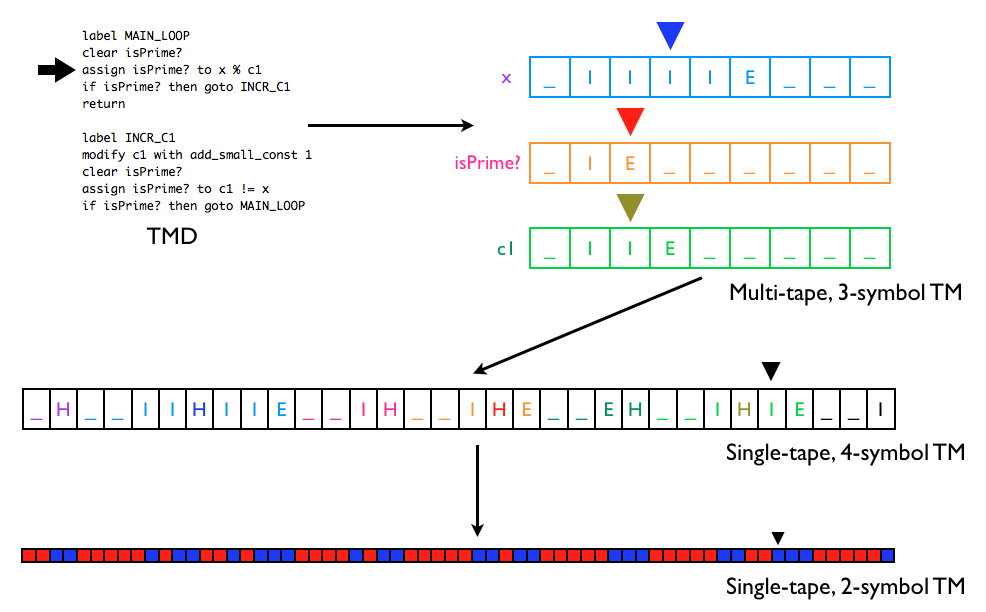
\includegraphics[height=3.25in,width=5in,angle=0]{figs/process.png} 
\caption{This diagram illustrates each of the steps in the conversion between a program written in TMD and a description of a single-tape Turing machine with a binary tape alphabet.\label{fig:process}} 
\end{center} 
\end{figure}  


The full Turing machine, along with the entirety of the TMD code that compiles down to it and the compiler itself, are available for public use at~\cite{github}.

\section{Major Design Decisions}

Our goal is ultimately to produce a \emph{parsimonious} Turing machine: a Turing machine with minimal number of states. The design of the compiler is informed by this fact. \\

\subsection{The Tape-Variable Relationship}

The first major design decision was to use the higher-level abstraction of a multi-tape Turing machine to represent the variables in a convenient manner. Later, the multi-tape Turing machine is automatically converted to a single-tape Turing machine.  \\

In the multi-tape Turing machine, each variable is given its own tape. This makes it easy to keep the variables separate. Allowing separate variables in the compiled language is crucial if we want to use standard programming techniques. \\

There are several possible definitions of the behavior of a multi-tape Turing machine that we could use. Perhaps the most common is the one in which each of the heads on each of the different tapes reads a symbol simultaneously, and each head is allowed to move right or left based on the combination of symbols that was read. Although this representation is powerful, it is expensive in terms of the number of states used: the number of lower-level states required is exponential in the number of tapes $t$ in the Turing machine, which in this case equals the number of variables in the TMD program. \\

Instead, I chose a representation that is slightly weaker but much more parsimonious. Each state $s$ in the higher-level multi-tape Turing machine has associated with it a single tape $T_s$. State transitions out of $s$ can only depend on the symbol read from $T_s$, and not on the symbols on the other tapes. In addition, after the symbol is read from $T_s$, only the tape head on $T_s$ can move left or right; other tapes' tape heads must remain in place. However, state transitions out of $s$ may go to states that are associated with other tapes. 

\subsection{Unary}

The second major design decision was to encode all integers in \emph{unary}: base-one notation. In other words, 1 is represented by ``\texttt{1},'' 2 is represented by ``\texttt{11},'' 3 by ``\texttt{111},'' etc. Numbers represented in unary take space linear in the value of the number being represented. As a result, the Turing machine produced by the compiler is exponentially slower and less space-efficient than it might have been with a more efficient numerical representation. However, it is also more parsimonious. Algorithms for computing arithmetic operations in unary are substantially simpler than their binary counterparts, and in this situation, simplicity is all that counts. \\

As an example, consider integer divison. In binary, a series of complicated subtractions must be done to compute $\left \lfloor{\frac{a}{b}}\right \rfloor$ in polynomial time. On a multi-tape Turing machine with the numbers written in unary, however, the problem becomes far simpler. If \texttt{a} is written on tape $T_a$ and \texttt{b} is written on tape $T_b$, and the output is expected to go on tape $T_c$, all that is necessary is to advance the heads on both $T_a$ and $T_b$ repeatedly. If the head on $T_b$ reaches the end of \texttt{b}'s representation, increment \texttt{c} and return the head on $T_b$ to the beginning of \texttt{b}. If the head on $T_a$ reaches the end of \texttt{a}'s representation, the algorithm terminates. \\

\subsection{Functions \label{sec:functions}}

The third major design decision was to allow function calls, but not recursion. In the compiler, functions are compiled in a way that is equivalent to \emph{inlining} every function and then compiling the resulting program. (To \emph{inline} a function means to splice the code of the function into the place that the function was called.) This means that a separate set of states needs to be made for every call of each function, because the function's return address has been ``hard-coded'' into the set of states, instead of stored on the tape. Note that using this design choice, recursive functions (functions that directly or indirectly call themselves) are impossible: to inline such a function would cause an infinite loop. \\

Another possible choice for function processing would be to write the function stack directly onto the tape. In other words, instead of creating a set of states for every function call, simply create a set of states for every function proper, and write the current line number and current function on the tape. Whenever a function call occurs, push a representation of the return address onto the stack on the tape. When a function returns, return to the return address written at the top of the stack and remove it. \\

Because this approach creates a set of states for every line of code written across any function, instead of a set of states for every line of code multiplied by the number of times the surrounding function is called, writing the stack onto the tape can potentially be exponentially more parsimonious. In particular, when the program contains $k$ subroutines $f_1, f_2, \dots, f_k$, and for each $1 \le i < k$, $f_i$ calls $f_{i+1}$ twice, the states associated with $f_k$ will appear $2^k$ times in the compiled Turing machine using the inlining method, but will only appear once using the stack-on-tape method. In addition, the stack-on-tape allows for the use of recursive functions.\\

In general, in the graph where each function in the program is given its own node, and where a directed edge is drawn from function $f_i$ to function $f_j$ for each time that $f_i$ calls $f_j$, the number of times that the code of $f_j$ will appear in the ultimate compiled program using the inlining method will be proportional to the number of paths from the main function to $f_j$ in the graph. Note that a recursive function corresponds to a cycle in the graph, and therefore to an infinite number of paths! Note, also, that even if the graph is acyclic, the number of paths to $f_j$ can potentially be exponential in the size of the graph. \\

What, then, is the advantage of the inlining method? Besides being easier to implement from the point of view of designing the compiler, the main advantage is that it avoids the overhead of writing the function stack and line number on the tape, and needing to read it each time a line of code is executed. Additionally, if each function is only ever called once, inlining is no worse than writing the stack on the tape. Because most of the functions in my program are only used once and are separated from each other mainly for the purpose of making testing easier, inlining was a natural choice. For a different application in which functions were going to be reused a lot, or in which recursive functions were very important or much simpler than using loops, writing the stack on the tape might have been a much better choice. \\

For a side-by-side comparison of how a compiled program would look using the inlining and the stack-on-tape methods, see Figs.~\ref{fig:code} and~\ref{fig:compiled}.

\begin{figure} 
\begin{center} 
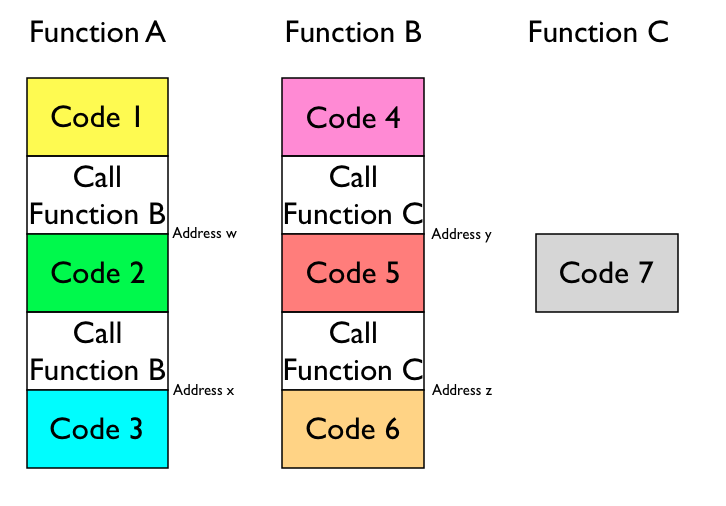
\includegraphics[scale=0.6]{figs/code.png} 
\caption{This is a visual representation of a program that spans three functions. The main function, Function A, calls Function B twice, and Function B calls Function C twice. Commands that are not function calls are labeled ``Code 1'' through ``Code 7.'' \label{fig:code}} 
\end{center} 
\end{figure}

\begin{figure} 
\begin{center} 
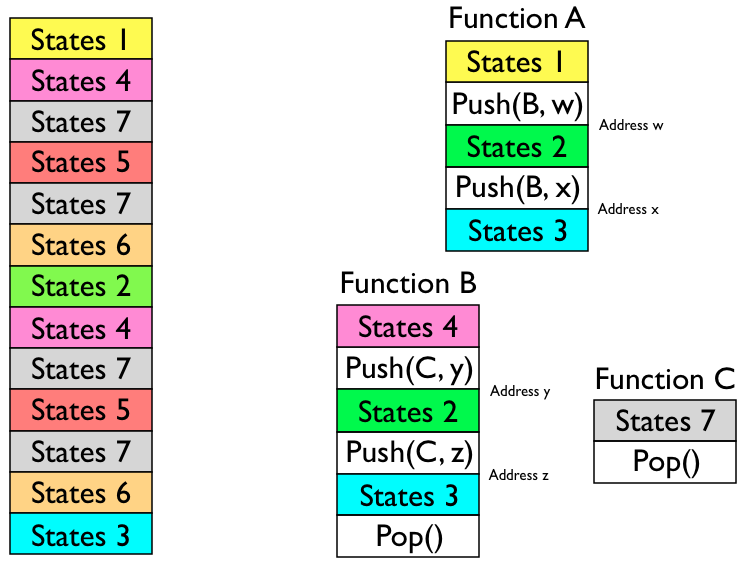
\includegraphics[scale=0.6]{figs/compiled.png} 
\caption{This is a visual representation of the compiled output of the program from Figure~\ref{fig:code}. On the left is the output of the compiler assuming the inlining method is used, while on the right is the output of the compiler assuming the stack-on-tape method is used. Note that the program flow of the compiled machine on the left is easier to understand; the program flow of the compiled machine on the right depends on what function is at the top of the stack. However, note also that if the set of states that represents ``Code 7,'' ``States 7,'' is very large, the stack-on-tape method is much more parsimonious than the inlining method in this case. On the left, ``States 7'' appears four times, but on the right it only appears once. \label{fig:compiled}} 
\end{center} 
\end{figure}

\section{Future Directions}

There are many improvements that could be made to the work in this thesis. The improvements can be separated into three categories, which are discussed in turn.

\subsection{Improving TMD}

TMD is a relatively weak language with many awkward aspects. For example, TMD does not support complex arithmetical expressions, either in assignment or as part of an \texttt{if} statement. Ideally, arbitrary expressions could be used in any of these places, to make TMD programs shorter. \\

Also, the fact that variables need to have a value of 0 before they can be reassigned is an annoyance. This aspect of TMD exists because sometimes the programmer already knows that the variable has a 0 value, so it would be wasteful to ``build in'' setting the value of the variable to 0 before reassignment. However, it would be more convenient if the compiler could automatically recognize most of the situations where the variable is guaranteed to have a 0 value (such as when it hasn't been touched since declaration) and automatically forgo clearing the variable's value in those situations. \\

Finally, it would be very nice if \texttt{while} and \texttt{for} loops were possible in TMD, to make programs cleaner and easier to read. While \texttt{goto} statements are natural from the point of view of simplicity of compilation, they tend to lead to to bad programming habits and inscrutable code. Providing programmers with the option of using \texttt{while} loops instead would make the job of debugging TMD programs easier. 

\subsection{Simplifying $Z$}

The final Turing machine, $Z$, whose behavior cannot be proven in ZFC, is not as parsimonious as it could be. At a basic level, the process of building a general-purpose compiler to Turing machines and then using that general-purpose compiler to create a specific program cannot possibly be as parsimonious as building the program directly. Abandoning the rigid abstraction barrier between the multi-tape and the single-tape abstraction, for example, would surely make the resulting program more parsimonious. However, this improvement in the number of states in the Turing machine comes at a tremendous cost in programmer effort. \\

Nonetheless, there are many more optimizations that are possible to reduce the number of states. To start with, writing the function stack on the tape and trying as much as possible to rewrite different functions to reuse the same code could potentially result in a savings in the number of states. Although we rarely call identical functions in the final program, there are many instances where we call two very similar functions at different points. When those functions are complex enough, it becomes worth it to build a single function capable of running both depending on its inputs, and calling that function twice with different arguments each time. Assuming the stack-on-tape method of compiling functions is used (see~\ref{sec:functions} for a description of this method), this will most likely result in the number of states in the final program being substantially reduced. \\

Also, making the compiler more parsimonious at each stage is a good way to improve the upper bound presented in this thesis. In particular, the transformation from a 4-symbol Turing machine to a 2-symbol Turing machine has possible improvements that would likely result in a reduction of state usage by a factor of 1.5 or more; see Section~\ref{sec:mstots} for the details on what can be improved in the behavior of that compiler. \\

\subsection{Exploring Other Axiomatic Systems}

There are many possible axiomatic systems that could have been used as ``the foundation of modern mathematics''; for most purposes, Peano Arithmetic (PA), a weaker axiomatic system than ZFC, is enough to prove interesting mathematical statements. Friedman has even conjectured that the still weaker system of Elementary Function Arithmetic (EFA) could be used to prove every theorem published in the \emph{Annals of Mathematics}.~\cite{grandconjecture}
This includes Fermat's Last Theorem, whose original proof involved \emph{Grothendieck universes}, which require stronger axioms even than ZFC. (See~\cite{grothendieck}) \\ 

It could therefore be interesting to find the upper bounds on the highest Busy Beaver values provable using these other systems of axioms--PA, EFA, and ZFC with Grothendieck universes. \\

This kind of further research would be helpful to give researchers a numerical value to assign to the complexity of various axiomatic systems. Friedman has helpfully created many relatively-easy-to-program statements, like Statement~\ref{eq:friedman},~\cite{friedmanlist} which cannot be proved in various axiomatic systems. The TMD compiler is well-suited to turning these statements into small Turing machines.

\section{TMD}

The top-level representation is a program written in the TMD language, which is a language created and designed explicitly for use in this project. TMD is not unlike Assembly Language, although it is more powerful in some ways and weaker in others. \\

TMD code can be processed in two ways. First, it can be \emph{interpreted}; that is, it can be directly evaluated line-by-line. This is generally done to verify a program's correct behavior, and to correct errors which would result in thrown exceptions in the interpreter but might lead to undefined behavior in the compiled Turing machine (because the compiled Turing machine is optimized for parsimony, whereas the interpreter need not be). \\

Second, TMD code can be \emph{compiled} down to a lower-level representation, such as a multi-tape, 3-symbol Turing machine, a single-tape, 4-symbol Turing machine, or a single-tape, 2-symbol Turing machine. It is highly recommended, however, to first interpret any piece of TMD code before compiling it, because the interpreter is much better for catching programming errors. The compiler is general-purpose and not restricted to compiling the programs discussed in this thesis; it could be valuable on its own, as a pedagogical tool. Naturally, the compiler is optimized to minimize the number of states in the resulting Turing machine, not to make the resulting Turing machine time- or space-efficient. \\

There are two types of TMD files. The first type of TMD file is a \emph{main file}, which can be run on its own, but cannot be called by another program. The second type of file is a \emph{function file}, which can be called by another program, but cannot be run on its own. The two types of files obey differing syntax, and the differences between them will be explained in further detail in this section. \\

A TMD program is a sequence of \emph{commands}. Commands are separated by newlines. Each command is given its own line. \\

\subsection{List of Commands}

The following is a list of possible commands. Let \texttt{x}, \texttt{x1}, \texttt{x2}, and \texttt{x3} be the names of distinct variables, let \texttt{c} be a numerical constant, and let \texttt{f} be the name of a function. Let \texttt{L} be the name of a code label. \\

\textbf{Main files only} \\ \\
\texttt{var x}: Declares a variable with the name \texttt{x}. \\ \\
\texttt{vars x1 x2} \dots: Declares several variables with the names \texttt{x1}, \texttt{x2}, \dots \\

\textbf{Function files only} \\ \\
\texttt{input x1 x2} \dots: Defines the arguments to the function file to be \texttt{x1}, \texttt{x2}, \dots \\ \\\
\texttt{return}: Exits the function and returns to executing wherever the function was called. \\

\textbf{Either file} \\ \\
\texttt{assign x1 to x2} [operation] \texttt{x3}: Changes the value of the variable \texttt{x1} to the result of \texttt{x2} [operation] \texttt{x3}. \\ \\
\texttt{assign x1 to x2} [operation] \texttt{c}: Changes the value of the variable \texttt{x1} to the result of \texttt{x2} [operation] \texttt{c}. \\ \\
\texttt{assign x1 to x2} [operation]: Changes the value of the variable \texttt{x1} to the result of the operation [operation] applied to \texttt{x2}. \\ \\
\texttt{assign x1 to x2}: Changes the value of the variable \texttt{x1} to the value of the variable \texttt{x2}, as long as \texttt{x2} is an \texttt{int}. \\ \\
\texttt{modify x1 with} [operation] \texttt{x2}: Changes the value of the variable \texttt{x1} to the result of \texttt{x1} [operation] \texttt{x2}. \\ \\
\texttt{modify x with} [operation] \texttt{c}: Changes the value of the variable \texttt{x} to the result of \texttt{x1} [operation] \texttt{x2}. \\ \\
\texttt{clear x}: Changes the value of the variable \texttt{x} to 0. \\ \\
\texttt{label L}: Declares a label L. \\ \\
\texttt{goto L}: Changes the line of code being executed to the line of code that contains ``\texttt{label L}.'' \\ \\
\texttt{if x goto L}: If the current value of \texttt{x} is a positive integer, then changes the line of code being executed to the line of code that contains ``\texttt{label L}.'' \\ \\
\texttt{function f x1 x2 x3} \dots: Calls the function \texttt{f} on input variables \texttt{x1}, \texttt{x2}, \texttt{x3}, \dots \\
\texttt{print x}: Prints the value of the variable \texttt{x}. Print statements only run if the program is being interpreted. \\ \\
\texttt{accept}: The Turing machine accepts. \\ \\ 
\texttt{reject}: The Turing machine rejects. 

\subsection{Main Files}

Main files contain the body of a program, and can be run. Any variable declared at any point in a main file will be initialized before the execution of the program, with an initial value of 0. As part of their execution, main files can call function files, but they cannot call other main files. Main files may not reach the end of the program without accepting or rejecting. \\

See Section~\ref{sec:mainfilegoldbach} for an example of a main file.

\subsection{Function Files}

Function files contain the description of a function. They cannot be run alone; instead, they are called from within a main file or another function file. \\
  
New variables may not be declared from within a function file; instead, any variables needed to perform the computation in the function file are passed from the file that calls it. Any variables passed into a function file may be modified freely, including integers; that means that there is \emph{no} built-in guarantee that inputs to a function will retain their values after the function runs. \\

Function files may not reach the end of the program without accepting, rejecting, or returning. When a function returns, execution continues at the location of the line beneath where the function was called. Functions never return values; instead, they work by modifying the inputs they are given. Although functions can be called by other functions, they cannot be called recursively (that is, they cannot call themselves and they cannot call functions that eventually call them). \\

See Section~\ref{sec:functionfilegoldbach} for an example of a function file.

\subsection{Data Types}

TMD has three data types: \texttt{int}, \texttt{list}, and \texttt{list2}. An \texttt{int} is a non-negative integer. A \texttt{list} is a list (possibly empty) of \texttt{int}s. A \texttt{list2} is a list (possibly empty) of \texttt{list}s. TMD is not strongly typed; a variable can at various points belong to different data types. In fact, it can even belong to multiple data types at once. The \texttt{int} value of \texttt{0}, the \texttt{list} value of \texttt{[]}, and the \texttt{list2} value of \texttt{[]} are all represented the same way on the Turing machine's tape. In accordance with this paradigm, even in the TMD interpreter, if the programmer chose to add \texttt{3} to a variable whose current value was \texttt{0}, it would yield the value \texttt{3}, but if the programmer chose instead to \emph{append} \texttt{3} to a variable whose current value was \texttt{0}, it would yield the value \texttt{[3]}. This is the only situation in which a variable can belong to several data types simultaneously.

\subsection{Assign Statements}

Assign statements can take any of the following four forms: \\ \\
\texttt{assign x1 to x2} [operation] \texttt{x3} \\ 
\texttt{assign x1 to x2} [operation] \texttt{c} \\
\texttt{assign x1 to x2} [operation] \\
\texttt{assign x1 to x2} \\

Assign statements result in the value of \texttt{x1} being set to the result of the operation [operation] being applied to \texttt{x2} and \texttt{x3} in the first case, to \texttt{x2} and \texttt{c} in the second case, and to \texttt{x2} alone in the third case. In the fourth case, the value of \texttt{x1} is set to the value of \texttt{x2}, as long as \texttt{x2} is an \texttt{int}. Unlike in most programming languages, the value of \texttt{x1} must be 0 before an assign statement can be applied to it. \\

Some assign statements involve constant arithmetic. These statements generally specify that the constant $c$ should be \emph{small}. This is because these statements give rise to $O(c)$ Turing machine states. For constants greater than about 20, it is better to assign a variable to take on the constant's value using interated multiplication, and use the standard arithmetic operation instead, using $O(\log c)$ states. For particularly enormous constants, it may even be advisable to construct a parsimonious function file simply to generate them using a function file; if the function file is very well-designed, this may take as few as $O(BB^{-1}(c))$ states! \\

In the explanations that follow, the value of \texttt{x1} is $x_1$, the value of \texttt{x2} is $x_2$, the value of \texttt{x3} is $x_3$, and the value of \texttt{c} is $c$. As before, \texttt{x1}, \texttt{x2}, and \texttt{x3} denote variables, and \texttt{c} denotes a numerical constant. Note that the allowed operations in assign statements are \emph{not} the same as the allowed operations in modify statements. This is because some operations are more parsimonious as an assignment, and other operations are more parsimonious as a modification.

\subsubsection{Multiplication}

\texttt{assign x1 to x2 * x3} \\
implements the operation $x_1 \leftarrow x_2 x_3$. \\ \\
$x_2$ and $x_3$ are required to be \texttt{int}s. \\
After this operation, $x_1$ is an \texttt{int}.

\subsubsection{Division} 

\texttt{assign x1 to x2 / x3} \\
implements the operation $x_1 \leftarrow \left \lfloor{\frac{x_2}{x_3}}\right \rfloor$. \\ \\
$x_2$ and $x_3$ are required to be \texttt{int}s. \\
After this operation, $x_1$ is an \texttt{int}.

\subsubsection{Modulus} 

\texttt{assign x1 to x2 \% x3} \\
implements the operation $x_1 \leftarrow x_2\mod x_3$. \\ \\
$x_2$ and $x_3$ are required to be \texttt{int}s. \\
After this operation, $x_1$ is an \texttt{int}.

\subsubsection{Integer Equality Testing}

\texttt{assign x1 to x2 = x3} \\
implements $x_1 \leftarrow 1$ if and only if $x_2 = x_3$. \\ \\
$x_2$ and $x_3$ are required to be \texttt{int}s. \\
After this operation, $x_1$ is an \texttt{int}.

\subsubsection{Integer Inequality Testing}

\texttt{assign x1 to x2 != x3} \\
implements $x_1 \leftarrow 1$ if and only if $x_2 \not= x_3$. \\ \\
$x_2$ and $x_3$ are required to be \texttt{int}s. \\
After this operation, $x_1$ is an \texttt{int}.

\subsubsection{Constant Equality Testing}

\texttt{assign x1 to x2 equals\_small\_const c} \\
implements $x_1 \leftarrow 1$ if and only if $x_2 = c$. \\ \\
$x_2$ is required to be an \texttt{int}.
After this operation, $x_1$ is an \texttt{int}.

\subsubsection{Comparison (Greater Than)}

\texttt{assign x1 to x2 > x3} \\
implements $x_1 \leftarrow 1$ if and only if $x_2 > x_3$. \\ \\
$x_2$ and $x_3$ are required to be \texttt{int}s. \\
After this operation, $x_1$ is an \texttt{int}.

\subsubsection{Comparison (Less Than)}

\texttt{assign x1 to x2 < x3} \\
implements $x_1 \leftarrow 1$ if and only if $x_2 < x_3$. \\ \\
$x_2$ and $x_3$ are required to be \texttt{int}s. \\
After this operation, $x_1$ is an \texttt{int}.

\subsubsection{List Equality Testing}

\texttt{assign x1 to x2 list\_equals x3} \\
implements $x_1 \leftarrow 1$ if and only if $|x_2| = |x_3|$ and for all integers $0 \le i < |x_2|$, the $i^{\textrm{th}}$ element of $x_2$ equals the $i^{\textrm{th}}$ element of $x_3$. \\ \\
$x_2$ and $x_3$ are required to be \texttt{list}s or \texttt{list2}s. \\
After this operation, $x_1$ is an \texttt{int}. 

\subsubsection{List Index}

\texttt{assign x1 to x2 index x3} \\
implements $x_1 \leftarrow v$, where $v$ is the $x_3^{\textrm{th}}$ value in $x_2$ (0-indexed). \\ \\
$x_2$ is required to be a \texttt{list}, and $x_3$ is required to be an \texttt{int}. \\
After this operation, $x_1$ is an \texttt{int}.

\subsubsection{List2 Index}

\texttt{assign x1 to x2 index2 x3} \\
implements $x_1 \leftarrow v$, where $v$ is the $x_3^{\textrm{th}}$ value in $x_2$ (0-indexed). \\ \\
$x_2$ is required to be a \texttt{list2}, and $x_3$ is required to be an \texttt{int}. \\
After this operation, $x_1$ is a \texttt{list}.

\subsubsection{List Length}

\texttt{assign x1 to x2 length} \\
implements $x_1 \leftarrow |x_2|$. \\ \\ 
$x_2$ is required to be a \texttt{list}. \\
After this operation, $x_1$ is an \texttt{int}.

\subsubsection{List2 Length} 

\texttt{assign x1 to x2 length2} \\
implements $x_1 \leftarrow |x_2|$. \\ \\  
$x_2$ is required to be a \texttt{list2}. \\
After this operation, $x_1$ is an \texttt{int}.

\subsubsection{List Assignment}

\texttt{assign x1 to x2 list} \\
implements $x_1 \leftarrow x_2$. \\ \\  
$x_2$ is required to be a \texttt{list} or \texttt{list2}. \\
After this operation, $x_1$ is a \texttt{list} or a \texttt{list2}.

\subsection{Modify Statements}

Modify statements can take either of the following two forms: \\ \\
\texttt{modify x1 with} [operation] \texttt{x2} \\ 
\texttt{modify x1 with} [operation] \texttt{c} \\

Modify statements result in the value of \texttt{x1} being set to the result of the operation [operation] being applied to \texttt{x1} and \texttt{x2} in the first case, and to \texttt{x1} and \texttt{c} in the second case. \\

In the explanations that follow, the value of \texttt{x1} is $x_1$, the value of \texttt{x2} is $x_2$, and the value of \texttt{c} is $c$. As before, \texttt{x1} and \texttt{x2} denote variables, and \texttt{c} denotes a numerical constant. Note that the allowed operations in assign statements are \emph{not} the same as the allowed operations in modify statements. This is because some operations are more parsimonious as an assignment, and other operations are more parsimonious as a modification.

\subsubsection{Addition}

\texttt{modify x1 with + x2} \\
implements the operation $x_1 \leftarrow x_1 + x_2$. \\ \\
$x_1$ and $x_2$ are required to be \texttt{int}s. \\
After this operation, $x_1$ is an \texttt{int}.

\subsubsection{Subtraction}

\texttt{modify x1 with - x2} \\
implements the operation $x_1 \leftarrow x_1 - x_2$. \\ \\
$x_1$ and $x_2$ are required to be \texttt{int}s. \\
After this operation, $x_1$ is an \texttt{int}.

\subsubsection{Constant Addition}

\texttt{modify x1 with add\_small\_const c} \\
implements the operation $x_1 \leftarrow x_1 + c$. \\ \\
$x_1$ is required to be an \texttt{int}. \\
After this operation, $x_1$ is an \texttt{int}.

\subsubsection{Constant Subtraction}

\texttt{modify x1 with sub\_small\_const c} \\
implements the operation $x_1 \leftarrow x_1 - c$. \\ \\
$x_1$ is required to be an \texttt{int}. \\
After this operation, $x_1$ is an \texttt{int}.

\subsubsection{Appending to Lists}

\texttt{modify x1 with append x2} \\
implements the operation $x_1 \leftarrow x_1 || [x_2]$, where $||$ denotes the concatenation operation. \\ \\
$x_1$ is required to be a \texttt{list}, and $x_2$ is required to be an \texttt{int}. \\
After this operation, $x_1$ is a \texttt{list}.

\subsubsection{Appending to List2s}

\texttt{modify x1 with append2 x2} \\
implements the operation $x_1 \leftarrow x_1 || [x_2]$, where $||$ denotes the concatenation operation. \\ \\
$x_1$ is required to be a \texttt{list2}, and $x_2$ is required to be a \texttt{list}. \\
After this operation, $x_1$ is a \texttt{list2}.

\subsubsection{Appending Constants}

\texttt{modify x1 with append\_small\_const c} \\
implements the operation $x_1 \leftarrow x_1 || [c]$, where $||$ denotes the concatenation operation. \\ \\
$x_1$ is required to be a \texttt{list}. \\
After this operation, $x_1$ is a \texttt{list}.

\subsubsection{List Concatenation}

\texttt{modify x1 with concat x2} \\
implements the operation $x_1 \leftarrow x_1 || x_2$, where $||$ denotes the concatenation operation. \\ \\
$x_1$ and $x_2$ are required to be \texttt{list}s. \\
After this operation, $x_1$ is a \texttt{list}.

\subsubsection{List2 Concatenation}

\texttt{modify x1 with concat2 x2} \\
implements the operation $x_1 \leftarrow x_1 || x_2$, where $||$ denotes the concatenation operation. \\ \\
$x_1$ and $x_2$ are required to be \texttt{list2}s. \\
After this operation, $x_1$ is a \texttt{list2}.

\subsection{Clear Statements}

Clear statements have the following form: \\ \\
\texttt{clear x} \\ \\ 
Clear statements implement the operation $x \leftarrow 0$. \\ \\
Clear statements are often used directly before an assignment to \texttt{x}, because assignment to \texttt{x} requires that $x = 0$. A clear statement can also be used to change the type of \texttt{x}, because \texttt{0} and \texttt{[]} are represented the same way on the Turing machine tape and are treated identically in TMD. Naturally, a clear statement can also be used if the programmer wants to set the value of \texttt{x} to 0. \\

\subsection{Label Statements}

Label statements have the following form: \\ \\ 
\texttt{label L} \\ \\
Label statements do nothing on their own. Instead, label statements \emph{mark} their line of code with their label. For instance, the label statement given above would mark its line of code with the label \texttt{L}. If at some later point, a \texttt{goto} statement is used on the label \texttt{L}, execution will \emph{jump} to whatever line of code contains ``\texttt{label L}.'' In other words, execution will continue at whichever line of code contains ``\texttt{label L}.'' \\ \\
Because label statements have no direct effect, they can also be used for comments. If multiple words follow the \texttt{label} word, all but the first is ignored (and the first becomes the label $L$). \\ \\
Programs cannot contain multiple declarations of the same label.

\subsection{Goto Statements}

Goto statements have the following form: \\ \\
\texttt{goto L} \\ \\ 
When a statement of this form is executed, code execution jumps to whichever line of code contains ``\texttt{label L}.''

\subsection{If-Goto Statements}

If-goto statements have the following form: \\ \\
\texttt{if x goto L} \\ \\ 
When a statement of this form is executed, code execution jumps to whichever line of code contains ``\texttt{label L}'' if \texttt{x} is an \texttt{int} with $x > 0$. If $x = 0$, or if \texttt{x} is a \texttt{list} or a \texttt{list2}, code execution continues to the next line like normal. \\

\subsection{Function Statements}

Function statements have the following form: \\ \\
\texttt{function f x1 x2 x3} \dots \\ \\ 
When a statement of this form is executed, code execution jumps to the top of the function file \texttt{f.tmd}. \texttt{f.tmd} must be in the same directory as whichever file called \texttt{f}. In addition, a mapping is created from the functions' variables to the variables in front of the function call. For example, calling \texttt{function f x1 x2 x3} when \texttt{f.tfn} contains at the top the line \texttt{input x4 x5 x6} will create a mapping from \texttt{x4} to \texttt{x1}, from \texttt{x5} to \texttt{x2}, and from \texttt{x6} to \texttt{x3}. In other words, any operation on \texttt{x4} in \texttt{f.tfn} will in fact be acting on \texttt{x1} from the file that made the function call. This mapping remains in effect until the function returns. \\

Functions cannot be called recursively. In other words, they cannot call themselves, or other functions that eventually call them. Formally, if each function was a node in a graph, and a directed edge was drawn from function \texttt{f1} to function \texttt{f2} if function \texttt{f1} called \texttt{f2}, then that graph cannot contain cycles.

\subsection{Print Statements}

Print statements have the following form: \\ \\ 
\texttt{print x} \\ \\ 
When a statement of this form is executed by the interpreter, ``\texttt{x:}''$|| x$ is printed to the standard output, where $x$ is a string representation of the value of \texttt{x} and $||$ is the string concatenation operation. Statements of this form are ignored by the compiler. Print statements are intended primarily to help debug a program that will later be compiled; the user need not worry about statements like these reducing the parsimony of the resulting compiled Turing machine, because the compiler ignores them during compilation.

\subsection{Halting Statements}

Halting statements have one of the following two forms: \\ \\
\texttt{accept} \\
\texttt{reject} \\ \\

Instructions like these instruct the Turing machine to halt and enter an accepting or a rejecting state, depending on which of these two commands was used. 

\subsection{Variable Declaration Statements}

Variable declaration statements have one of the following two forms: \\ \\
\texttt{var x1} \\
\texttt{vars x1 x2 x3} \dots \\

Variable declaration statements can only be used in main files. In function files, if more variables are required, more variables need to be passed in as arguments to the function. \\

Regardless of their location in the program, variable declaration statements act at the initialization of the program only, and are otherwise ignored. At the initialization of the program, each variable declaration statement acts to initialize each declared variable with a value of 0. In the compiled program, the number of variables declared indicates to the compiler how many tapes to initialize. \\

Depending on the programmer's preference, variables can be declared one at a time with a sequence of \texttt{var} statements, or all at once with a \texttt{vars} statement (or with a mix of the two). Behavior is identical in both cases.

\subsection{Function Input Statements}

Function input statements have the following form: \\ \\
\texttt{input x1 x2 x3} \dots \\

A function input statement defines the variables used in a function. In concert with the function call, it also defines a mapping from the names of the variables defined in the input statement to the variable names used in the function call. For example, calling \texttt{function f x1 x2 x3} when \texttt{f.tfn} contains at the top the line \texttt{input x4 x5 x6} will create a mapping from \texttt{x4} to \texttt{x1}, from \texttt{x5} to \texttt{x2}, and from \texttt{x6} to \texttt{x3}. In other words, any operation on \texttt{x4} in \texttt{f.tfn} will in fact be acting on \texttt{x1} from the file that made the function call. This mapping remains in effect until the function returns. \\

Function input statements must appear exactly once in every function file, as the first line of the program. Function input statements may not appear in main files.

\subsection{Return Statements}

Return statements have the following form: \\ \\
\texttt{return} \\

A return statement instructs code execution to exit the function it is currently in and to return to the line below where the function was originally called. Return statements may not appear in main files.

\section{Writing a TMD Program that is Independent of ZFC}

In order to write a TMD program that is independent of ZFC, I wrote a program that halts if and only if Statement~\ref{eq:friedman} is false. For convenience, I have duplicated Statement~\ref{eq:friedman} here: \\

\begin{statement} \label{eq:friedman2}
For all $k, n, r \ge 0$, every order invariant graph on $[Q]^{\le k}$ has a free $\{x_1,\dots,x_r, \\
ush(x_1),...,ush(x_r)\}$ of complexity $\le (8knr)!$, each $\{x_1, \dots, x_{(8kni)!}\}$
reducing $[x_1 \cup \dots \cup x_i \cup \{0,\dots,n\}]^{\le k}$. \cite{friedman}
\end{statement}

\subsection{Missing Data Types}

The first apparent problem is that at first glance, TMD does not appear to support the necessary data structures to encode Statement~\ref{eq:friedman}. Statement~\ref{eq:friedman} requires us to iterate over every rational number of complexity at most $(8knr)!$, which requires both fractions and negative numbers, neither of which are explicitly supported by TMD. Recall that the only numerical data type in TMD is the \texttt{int}, which is restricted to non-negative integers (due to ease of unary representation).\\

In the TMD program that I wrote, I obviated the need for fractions simply by multiplying every number in the statement by $((8knr)!)!$. Because a number of complexity $(8knr)!$ is a number which can be represented by a fraction whose numerator and denominator both have absolute value at most $(8knr)!$, multiplying a number of complexity $(8knr)!$ by $((8knr)!)!$ is guaranteed to yield an integer. This is because $((8knr)!)!$ is an integer multiple of every number less than or equal to $(8knr)!$. \\

In the TMD program I wrote, I represented signed numbers $s$ with pairs $(p, n)$ of positive integers, where at all times the value $s$ is presumed equal to $p - n$. Even though $p$ and $n$ are required to be non-negative, the resulting signed value can take on any value, positive or negative. This representation is, of course, highly redundant; however, it has the advantage that it makes addition, multiplication, and comparison of signed values very easy.

\subsection{Program Sketch}

The program iterates over all possible values of $k$, $n$, and $r$ by using the technique of \emph{dovetailing}: it sets a fourth variable, $l$, that it iteratively increases, and tries all values of $k$, $n$, and $r$ such that $k, n, r < l$ for each $l$. \\

For each possible set of values of $k$, $n$, and $r$, the program then creates every possible order invariant graph. It does this by first generating every integer of the form $a / b * ((8knr)!)!$, where $a$ and $b$ are integers that range from 0 to $(8knr)!$. It then sorts every integer of this form from least to greatest, and generates all ${((8knr)!)^2 \choose i}$ different possible vertices of size $i$, for each $i \le k$. Finally, it associates with this set of vertices an \emph{order invariance relation}: a list of tuples, each containing only the symbols $\{<, >, =\}$. Each tuple specifies a possible legal ordering for the elements of the vertices to obey. To give a few examples, the earlier-mentioned order invariant graph that has an edge from $a = (a_1, a_2)$ to $b = (b_1, b_2)$ if and only if $a_1 < b_1 < a_2 < b_2$ would have associated with it the order invariance relation $[(<, >, <, >)]$, which specifies that the smallest element of the two vertices must come from $a$, the next smallest must come from $b$, the next smallest must come from $a$, and so on. The graph with no edges would have associated with it the order invariance relation $[]$, and the complete graph would have associated with it the list containing every possible tuple. \\

For each of these order invariance relations, there is a corresponding order invariant graph. The order invariant graph is then checked to have a free $\{x_1,\dots,x_r, ush(x_1),...,ush(x_r)\}$ satisfying the condition that each $\{x_1, \dots, x_{(8kni)!}\}$ reduces $[x_1 \cup \dots \cup x_i \cup \{0,\dots,n\}]^{\le k}$. If no such set of vertices exists in the order invariant graph, the Turing machine halts. \\

This is checked simply by trying all $({((8knr)!)^2 \choose i})^r$ different ordered sets of $r$ vertices, and if any of them have the property that they are an independent set and that each of their subsets $\{x_1, \dots, x_{(8kni)!}\}$ reduces $[x_1 \cup \dots \cup x_i \cup \{0,\dots,n\}]^{\le k}$, then the Turing machine continues to the next order invariant graph. If none of the ordered sets have these two properties, the order invariant graph violates the property guaranteed by Statement~\ref{eq:friedman}, and the Turing machine halts. \\

The program itself can be found at~\cite{github}.

\section{Compilation from TMD to a Multi-Tape Machine} \label{sec:turdtotm}

This section is devoted to describing the algorithm used to compile a TMD program into a multi-tape, 3-symbol Turing machine.

\subsection{Turing Machine Format}

The following is an example of the file format of the multi-tape, 3-symbol Turing machine output by the compiler. \\

Let us suppose that the Turing machine has three states and two tapes. The three symbols in the Turing machine's alphabet are "\texttt{\_}," "\texttt{1}," and "\texttt{E}." The first state's name is "\texttt{StateOne}," the second state's name is "\texttt{StateTwo}," and the third state's name is "\texttt{StateThree}." The first tape's name is "\texttt{TapeA}," and the second tape's name is "\texttt{TapeB}." \\

\texttt{StateOne} is associated with \texttt{TapeA}. \texttt{StateTwo} is associated with \texttt{TapeB}. \texttt{StateThree} is associated with \texttt{TapeA}. \\

Each line defining the Turing machine's behavior in a given state is written as follows: \\

\texttt{[symbol read] -> [next state]; [direction]; [symbol written]} \\

In the actual Turing machine text file, [next state] is replaced by the state that the Turing machine would enter if it read the symbol [symbol read], [direction] is one of \{\texttt{R, L, -}\} and indicates the direction the head would move in, and [symbol written] is one of \{\texttt{\_, 1, E}\} and indicates the symbol that is written on the tape. Note that in the higher-level, multi-tape 3-symbol Turing machine, as indicated by the \texttt{-} symbol, the head can remain in place, (unlike the lowest-level Turing machine around which the Busy Beaver function is defined, where it cannot). \\

Figure~\ref{fig:tmexample} shows an example of such a Turing machine file. Figure~\ref{fig:behavior} gives a step-by-step depiction of the behavior of this Turing machine for five steps. \\

\begin{figure} 
\begin{center} 
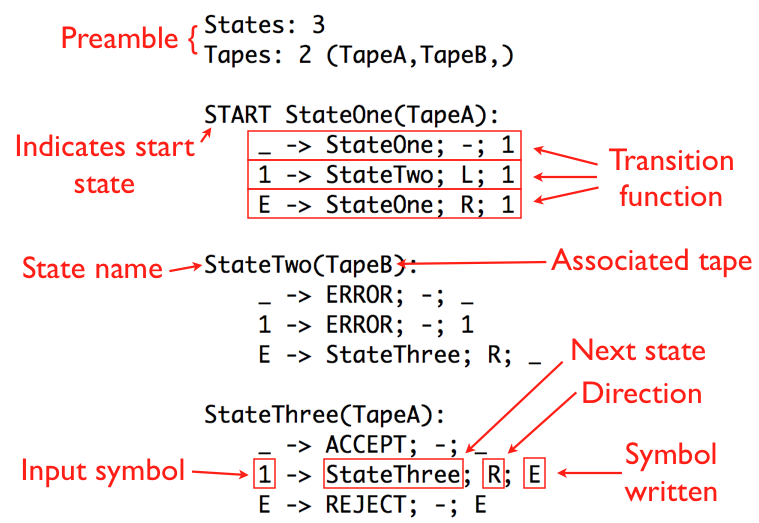
\includegraphics[scale=0.4]{figs/annotatedtm.png} 
\caption{This is an example of a multi-tape Turing machine file. The notes in red are explanations of the meanings of the various parts of the Turing machine file. \label{fig:tmexample}} 
\end{center} 
\end{figure}

\begin{figure} 
\begin{center} 
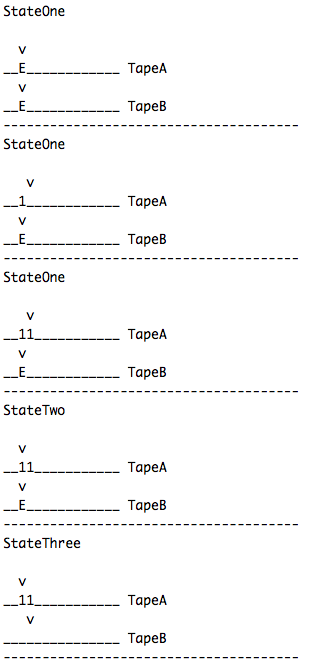
\includegraphics[scale=0.8]{figs/behavior.png} 
\caption{The machine of Figure~\ref{fig:tmexample} running for five steps. Note that in the multi-tape machine, at initialization, every tape begins with a single \texttt{E} symbol and an infinite number of \texttt{\_} symbols. As will be explained later, this corresponds to every variable having its value be initialized to 0. Naturally, in the lowest-level machine, the tape will be initialized containing only the empty symbol, as required of a standard Turing machine. \label{fig:behavior}} 
\end{center} 
\end{figure}

\subsection{Variable Encoding}

\indent Most of the work in compiling a TMD program to a description of a multi-tape Turing machine involves encoding the values of variables. As described earlier, each variable is given its own tape. \\

Because the empty tape symbol is \texttt{\_}, there will at all times be an infinite number of \texttt{\_} symbols on the tape. Therefore, all of the interesting information on the tape must come before the last appearing non-\texttt{\_} symbol. In every encoding of a value on the tape, it is guaranteed that the last appearing non-\texttt{\_} symbol is the \texttt{E} symbol. It is also guaranteed that there are no \texttt{\_} symbols that appear in between two non-\texttt{\_} symbols. In other words, the tape is guaranteed to have the following form: $(\texttt{\_})^\infty(\texttt{1}|\texttt{E})^*\texttt{E}(\texttt{\_})^\infty$. These two guarantees will be important in the transformation of the multi-tape machine to a single-tape machine (later, the \texttt{\_} symbol will serve as a separator symbol between different tapes). For the time being, however, these two guarantees serve mainly to constrain the form of the encoding. \\

Integer values are encoded in unary. Specifically, a value of \texttt{0} is encoded with \dots\texttt{\_\_E\_\_}\dots, a value of \texttt{1} is encoded with \dots\texttt{\_\_1E\_\_}\dots, a value of \texttt{2} is encoded with \dots\texttt{\_\_11E\_\_}\dots, and in general a value of $n$ is encoded with $(\texttt{\_})^\infty(\texttt{1})^n\texttt{E}(\texttt{\_})^\infty$. \\

List values are encoded as a sequence of numbers written in unary and broken by \texttt{E} symbols. Specifically, a value of \texttt{[]} is encoded with \dots\texttt{\_\_E\_\_}\dots (note the overlap with the encoding of \texttt{0}), a value of \texttt{[0]} is encoded with \dots\texttt{\_\_E\_\_}\dots, a value of \texttt{[2]} is encoded with \dots\texttt{\_\_E11E\_\_}\dots, and a value of \texttt{[3, 0, 2]} is encoded with \dots\texttt{\_\_E111EE11E\_\_}\dots. In general, a value of $[n_1, n_2, n_3, \dots n_k]$ is encoded with $(\texttt{\_})^\infty\texttt{E}(\texttt{1})^{n_1}\texttt{E}(\texttt{1})^{n_2}\texttt{E}(\texttt{1})^{n_3}\texttt{E}\dots(\texttt{1})^{n_k}\texttt{E}(\texttt{\_})^\infty$. \\

List2 values (lists of lists) are more challenging to encode than lists, because there is not an additional symbol which can be used to break apart the values for lists. The most natural first try is to use \texttt{E} to break between values within a list, and \texttt{EE} to break between different lists. This, however, lends itself to ambiguity, because the \texttt{EE} pattern appears naturally in simple lists that contain \texttt{0}. As an example, using that encoding scheme would result in the same representation for the \texttt{list2} value \texttt{[[3], [2]]} and the \texttt{list2} value \texttt{[[3, 0, 2]]}. \\

In order to fix this issue, the on-tape encoding of \texttt{list2} values increments every stored \texttt{int} value by 1, so that the \texttt{EE} pattern appears only when there is a break between stored \texttt{list}s, and not when a \texttt{list} contains a \texttt{0}. To give a few examples, a value of \texttt{[]} is encoded with \dots\texttt{\_\_E\_\_}\dots, a value of \texttt{[[3, 0], [1, 2]]} is encoded with \dots\texttt{\_\_E1111E1EE11E111EE\_\_}\dots, a value of \texttt{[[]]} is encoded with \dots\texttt{\_\_EE\_\_}\dots, and a value of \texttt{[[2, 4], [], [0]]} is encoded with \dots\texttt{\_\_E111E11111EEE1EE\_\_}\dots. In general, a value of $[[n^1_1, n^1_2, \dots, n^1_{k_1}], [n^2_1, n^2_2, \dots, n^2_{k_2}], \dots, [n^l_1, n^l_2, \dots, n^l_{k_l}]]$ is encoded with: $$(\texttt{\_})^\infty\texttt{E}(\texttt{1})^{n^1_1 + 1}\texttt{E}(\texttt{1})^{n^1_2 + 1}\texttt{E}\dots(\texttt{1})^{n^1_{k_1} + 1}\texttt{EE}(\texttt{1})^{n^2_1 + 1}\texttt{E}(\texttt{1})^{n^2_2 + 1}\texttt{E}\dots(\texttt{1})^{n^2_{k_2} + 1}\texttt{EE}\dots(\texttt{1})^{n^l_1 + 1}\texttt{E}(\texttt{1})^{n^l_2 + 1}\texttt{E}\dots(\texttt{1})^{n^l_{k_l} + 1}\texttt{EE}(\texttt{\_})^\infty$$

\subsection{Compilation \label{compilation}}

Compilation itself is a relatively straightforward matter. Lines of code correspond neatly to a single state or a group of states. In between two lines of code, the heads of all involved tapes are required to return to the position of the leftmost non-\texttt{\_} symbol, to retain consistency between situations in which a given line of code may be used. \\

To give an example, the line: \\
 
\texttt{if x goto L} \\

\noindent would correspond to a single state. That state would read the symbol underneath the head associated with \texttt{x}, and if that symbol was a \texttt{1}, the next state would be the first non-empty group of states reached after the line of code containing ``\texttt{label L}.'' If that state was an \texttt{E}, the next state would instead be the first non-empty group of states reached after the line of code below this one.\\

Many lines of code correspond to empty sets of states. For example, \texttt{label} statements, \texttt{goto} statements, variable declaration statements, input statements, and function calls all have empty sets of states associated with them. Such lines of code have no effect on compilation, other than to draw a pointer from the exit states of one set of states to the entrance state of another set of states. \\

The different possible sets of states associated with each possible line of code are too numerous for all of them to be described in detail in this paper. However, to give an example of what a more sophisticated set of states might look like, I present in Figure~\ref{fig:goldbach3} the state machine associated with the line: \\ \\
\texttt{assign x to y \% z} \\

\section{Transforming a Multi-Tape Machine to a Single-Tape Machine \label{sec:mttost}}

The output of the compiler described in Section~\ref{sec:turdtotm} is a description of a multi-tape Turing machine. Each state in the description has associated with it a tape, and in that state, only that tape is read and modified. We next present an algorithm for parsimoniously transforming such a multi-tape Turing machine into a single-tape Turing machine. \\

It is well-known that multi-tape Turing machines are ``equivalent'' to single-tape Turing machines in the sense that one can simulate the other assuming that an arbitrary overhead in terms of the number of states is allowable. This part of the thesis gives an explicit algorithm for simulating a multi-tape Turing machine using a single-tape Turing machine, which additionally tries to \emph{minimize} the overhead in the number of states. \\

In the descriptions that follow, to avoid confusion between the higher-level tapes of the multi-tape Turing machine and the lower-level tape of the single-tape Turing machine, the higher-level tapes are referred to as \emph{mini-tapes} and the single lower-level tape is referred to as the \emph{meta-tape}. \\

The transformation described below results in an overhead of about a factor of 5 in the number of states used in the machine (the exact overhead depends in part on the number of tapes in the multi-tape machine). 

\subsection{Alphabet}

The single-tape machine's alphabet consists of the three symbols from the multi-tape machine, \texttt{\_}, \texttt{1}, and \texttt{E}, and a new fourth symbol, \texttt{H}. \texttt{H} was introduced in order to be used as a stand-in for the head locations in each of the mini-tape values.

\subsection{Layout}

The transformation from a multi-tape Turing machine to a single-tape Turing machine must necessarily, from an information-theoretic standpoint, store all of the information on each of the many tapes of the multi-tape machine on the single tape. It also must store an identifier of which tape is which. \\

This directly implies what the approximate layout of the single-tape Turing machine must look like. Figure~\ref{fig:stmstmlayout} shows the high-level layout of the Turing machine's tape, along with a lower-level representation that will be explained in more detail in the following paragraphs. \\

As shown in Figure~\ref{fig:stmstmlayout}, the single tape is occupied by alternating identifiers and values. These identifiers and values are each separated by instances of the \texttt{\_} symbol (which also happens to be the empty symbol). Because the \texttt{\_} symbol is used as a separator and as an indicator that an identifier or a value has been read, the \texttt{\_} is not used inside the identifiers or the values proper. Therefore, identifiers and values draw only from the set of symbols \{\texttt{1}, \texttt{H}, \texttt{E}\}. \\

The last non-\texttt{\_} on the meta-tape is a \texttt{1}. The only time the \texttt{1\_} pattern appears on the tape signals that the last information on the tape has been read. This will be useful later when attempting to scan the entire tape for a specific value.

%\begin{figure} 
%\begin{center} 
%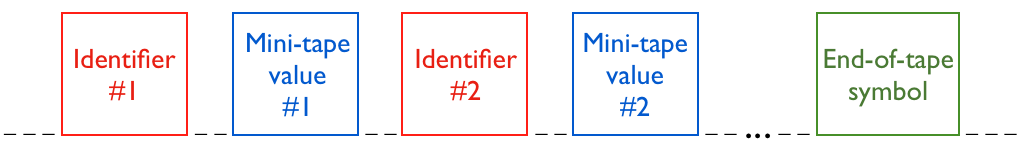
\includegraphics[scale=0.8]{figs/stmstmlayout.png} 
%\caption{A high-level representation of the information on the meta-tape. The information alternates between mini-tape identifier and mini-tape value. \label{fig:stmstmlayout}} 
%\end{center} 
%\end{figure}

\begin{figure} 
\begin{center} 
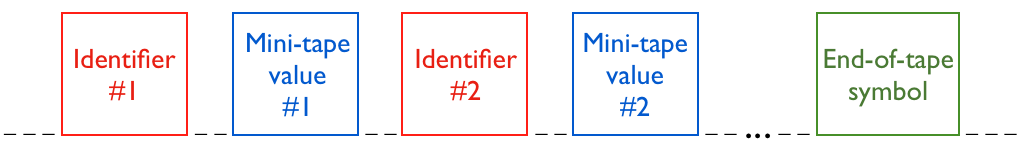
\includegraphics[scale=0.4]{figs/stmstmlayout.png} 
\caption{A high-level representation of the information on the meta-tape. The information alternates between mini-tape identifier and mini-tape value. \label{fig:stmstmlayout}}
\end{center} 
\end{figure}

\subsection{Identifier Format}

Identifiers are sequences of symbols drawn from \{\texttt{1}, \texttt{H}, \texttt{E}\} that indicate which mini-tape the value to the right of the identifier corresponds to. In other words, the compiler assigns to each mini-tape in the multi-tape Turing machine a unique sequence of \texttt{1}'s, \texttt{H}'s, and \texttt{E}'s. On the meta-tape, to the right of the sequence corresponding to a given mini-tape is that mini-tape's value. \\

On the meta-tape, the \texttt{H\_} pattern indicates the end of an identifier. Therefore, the last non-\texttt{\_} symbol in a valid identifier \emph{must} be \texttt{H}. However, the symbols preceding \texttt{H} in the identifier may be any of \texttt{H}, \texttt{E}, and \texttt{1}, and there may be any number of them. This means that in order to give each variable a unique identifier while making the lengths of identifiers as short as possible and while making the last symbol in each identifier an \texttt{H}, mini-tape identifiers should conform to the following pattern: \\ \\
Mini-tape 1: \texttt{H} \\
Mini-tape 2: \texttt{1H} \\
Mini-tape 3: \texttt{EH} \\
Mini-tape 4: \texttt{HH} \\
Mini-tape 5: \texttt{11H} \\
Mini-tape 6: \texttt{1EH} \\
Mini-tape 7: \texttt{1HH} \\
Mini-tape 8: \texttt{E1H} \\
Mini-tape 9: \texttt{EEH} \\
Mini-tape 10: \texttt{EHH} \\
\dots \\

Having access to three different symbols makes representing mini-tape identifiers as ternary numbers natural. Because there is also flexibility in the size of the number, however, it is best to use every 0-trit ternary number, followed by every 1-trit ternary number, followed by every 2-trit ternary number, and so on. \\

One natural question is: why should identifiers be as short as possible? After all, values in the Turing machine are represented in unary, which is far from the most concise way to represent a number. What motivates the different treatment of identifiers, which are represented in ternary, and values, which are represented in unary? \\

The answer is that the two types of sequences are treated very differently. Values are manipulated, and can often have many different possible values. If one is reading an integer $x$ with a value between 1 and $n$, and one wishes to behave differently for each possible value of $x$, one needs $\Omega(n)$ states to read in $n$'s value, no matter what number system is used to represent $x$. \\

By contrast, identifiers are generally scanned to see if they are equal to a specific value. If one is reading an integer $x$ with a value between 1 and $n$, and one is only interested in whether or not $x = k$ for some specific other value $k$, then there are only two possible outcomes: $x = k$ or $x \not= k$. This means that if $x$ is represented in base 2 or greater, it will be possible to determine which of $x = k$ or $x \not= k$ is true using only $O(\log k)$ states. \\

\subsection{Value Format}

Values are sequences of symbols drawn from \{\texttt{1}, \texttt{H}, \texttt{E}\}. They are meant to represent faithfully the information contained on each mini-tape. Because information on mini-tapes is entirely composed of \texttt{1} and \texttt{E} symbols (although the \texttt{\_} symbol appears on the mini-tapes, it never appears in between two non-\texttt{\_} symbols), the most natural way to represent the information on the mini-tape on the meta-tape is simply to write the symbols from the mini-tape directly onto the meta-tape. \\

This approach successfully records all of the information on the mini-tape except for one part: the location of the mini-tape's head (which I will refer to from now on as the \emph{mini-head}). Recall that each mini-tape has its own head, that state transitions are possible between states associated with two different mini-tapes, and that each mini-head's location must be remembered in between transitions. This was abstracted away by the higher-level Turing machine representation before, when we assumed that we could have many different tapes and one head for each of them. Now that we are trying to do everything on a single tape, however, we have only one head to go around. \\

The solution to this issue is the \texttt{H} symbol. The \texttt{H} symbol is always kept immediately to the left of the symbol over which the tape's mini-head would be. Because each mini-tape has only one head, there can only be one \texttt{H} symbol in a mini-tape value at once, the location of which represents the mini-head's location. The mini-tape value representation on the meta-tape is otherwise symbol-for-symbol identical to the sequence of symbols on the higher-level mini-tape.

\subsection{Value Expansion}

The diagram in Figure~\ref{fig:stmstmlayout} obscures a detail that complicates this transformation. The issue is that although the diagram appears to allocate a fixed block of the meta-tape to each identifier and each mini-tape value, no fixed number of tape slots can suffice to hold a mini-tape value. Because tape identifiers are static (they are drawn on the tape at initialization and never changed again), tape identifiers can be contained in a fixed number of tape slots. Mini-tape values, however, can get arbitrarily large; this means that they potentially need an arbitrarily large amount of space allocated to them. \\

The solution is to dynamically increase the space allocated to a mini-tape value whenever the mini-tape value increases in size. In other words, whenever a state in the multi-tape Turing machine is instructed to write a non-\texttt{\_} symbol on top of a \texttt{\_} symbol, it enters a group of intermediate states designed to ``push'' every symbol down along the tape, to create one more symbol of room for the mini-tape value. This group of intermediate states remembers the symbol it just read, moves right, writes down the symbol it just read, and repeats. See Figure~\ref{fig:goldbach4} for a diagram of the state machine used to ``push'' every symbol along the tape and make room for the expanding mini-tape value. \\

\subsection{Overview of Transformation \label{mttoststeps}}

Now that the high-level ideas have been described in detail, a step-by-step low-level description of the transformmation process can be given. \\

Suppose that the multi-tape Turing machine contains an instruction of the form: \\

\emph{When in State $S_a$ (associated with Tape $T_a$), if symbol $r$ is read, write the symbol $w$ on the tape, move the head in direction $d$, and enter State $S_b$ (associated with Tape $T_b$).} \\

In the single-tape Turing machine, this instruction will take many more states to represent, and will follow one of the series of instructions below, depending on the values of $r$, $w$, $T_a$, and $T_b$. \\

\textbf{If $r = \texttt{\_}$ and $w \not= \texttt{\_}$:}

\begin{enumerate}

\item Read the symbol below the meta-head. If that symbol is $r$, write $w$.
\item If the $d$ is an instruction not to move the mini-head, do nothing. Otherwise, swap the \texttt{H} symbol on the tape with the symbol to its left or right, depending on whether $d$ is ``left'' or ``right.''
\item Go right until the first \texttt{\_} symbol is found. Write a \texttt{\_} symbol onto the tape, and ``push'' every symbol to the right down one space on the meta-tape by remembering the symbol that was just read, moving right, writing the remembered symbol, and repeating. Do this until the \texttt{1\_} pattern is encountered, which signals the end of the information on the meta-tape.
\item Move the meta-head left, scanning for the sequence of symbols that corresponds to the identifier for tape $T_b$.
\item After the identifier has been reached, move the meta-head right until the \texttt{H\_} pattern is encountered, which signals the end of the identifier.
\item Move the meta-head right until the \texttt{H} symbol is encountered, which indicates the head is one symbol to the right. Move the meta-head right once more.

\end{enumerate}

\textbf{If $r \not= \texttt{\_}$ or $w = r$, and also $T_a \not= T_b$:}

\begin{enumerate}

\item Read the symbol below the meta-head. If that symbol is $r$, write $w$.
\item If the $d$ is an instruction not to move the mini-head, do nothing. Otherwise, swap the \texttt{H} symbol on the tape with the symbol to its left or right, depending on whether $d$ is ``left'' or ``right.''
\item Move the meta-head right until the \texttt{1\_} pattern is encountered, which signals the end of the information on the meta-tape.
\item Move the meta-head left, scanning for the sequence of symbols that corresponds to the identifier for tape $T_b$.
\item After the identifier has been reached, move the meta-head right until the \texttt{H\_} pattern is encountered, which signals the end of the identifier.
\item Move the meta-head right until the \texttt{H} symbol is encountered, which indicates the head is one symbol to the right. Move the meta-head right once more.

\end{enumerate}

\textbf{If $r \not= \texttt{\_}$ or $w = r$, and also $T_a = T_b$} (this case is special because the meta-head need not leave the mini-tape representation that it started on):
\begin{enumerate}

\item Read the symbol below the meta-head. If that symbol is $r$, write $w$.
\item If the $d$ is an instruction not to move the mini-head, do nothing. Otherwise, swap the \texttt{H} symbol on the tape with the symbol to its left or right, depending on whether $d$ is ``left'' or ``right.'' After swapping, move the meta-head one symbol to the right of the new \texttt{H} symbol.

\end{enumerate}

\section{Transforming a 4-Symbol Machine to a 2-Symbol Machine \label{sec:mstots}}

The output of the transformation process presented in Section~\ref{sec:mttost} is a description of a 4-symbol Turing machine. By contrast, the standard definition of the Busy Beaver function requires the alphabet to contain only two symbols. This means that an additional transformation step is necessary to turn the 4-symbol Turing machine into a 2-symbol machine. \\

Like the transformation described in Section~\ref{sec:mttost}, the equivalence of Turing machines with differently-sized finite alphabets is well-known. Unlike the transformation described in Section~\ref{sec:mttost}, common proofs of their equivalence tend to use the same techniques as the one described here. The general idea is to assign to each symbol in the larger alphabet an equivalent sequence of symbols in the smaller alphabet. \\

The transformation described below results in an overhead of about a factor of 20 in the number of states used in the machine.

\subsection{Alphabet}

The alphabet of the 2-symbol machine contains two symbols, which I decided to call \texttt{a} and \texttt{b}, because they don't map neatly to \texttt{0} and \texttt{1}, and because the \texttt{1} symbol was already used in the 4-symbol alphabet. \\

The mapping from \{\texttt{\_}, \texttt{1}, \texttt{H}, \texttt{E}\} to sequences of symbols from \{\texttt{a}, \texttt{b}\} is as follows: \\ \\
\texttt{\_} $\leftrightarrow$ \texttt{aa} \\
\texttt{1} $\leftrightarrow$ \texttt{ab} \\
\texttt{H} $\leftrightarrow$ \texttt{ba} \\
\texttt{E} $\leftrightarrow$ \texttt{bb} \\

\texttt{a} is the empty symbol.

\subsection{Overview of Transformation \label{sec:mstotssteps}}

The following is a step-by-step low-level description of the transformation process. \\

Suppose that the 4-symbol Turing machine contains an instruction of the form: \\

\emph{When in State $S_a$, if symbol $r$ is read, write the symbol $w$ on the tape, move the head in direction $d$, and enter State $S_b$.} \\

In the 2-symbol Turing machine, this instruction will take many more states to represent, and will follow one of the series of instructions below, depending on the values of $r$ and $w$. \\

\textbf{If $r = w$:}

\begin{enumerate}

\item Read the symbol below the head. Remember the symbol that was read, move right, and read the new symbol that is under the head. 
\item If the two symbols read in map to $r$, move three spaces left, one space left, or one space right, depending on whether $d$ is an instruction to move left, stay in place, or move right, respectively.

\end{enumerate}

\textbf{If $r \not= w$:}

\begin{enumerate}

\item Read the symbol below the head. Remember the symbol that was read, move right, and read the new symbol that is under the head.
\item Let $w_1$ be the first symbol in the sequence of symbols that that map to $w$, and let $w_2$ be the second symbol in that same sequence. If the two symbols read in map to $r$, write $w_2$, move left, and write $w_1$.
\item Move two spaces left, move left and then right, or move two spaces right, depending on whether $d$ is an instruction to move left, stay in place, or move right, respectively.

\end{enumerate}

Note that although the higher-level Turing machines with more than 2-symbol alphabets allow the head to stay in place, the bottom-most representation does not, which is important: in the standard definition of the Busy Beaver function, the head must move left or right at each step and cannot stay in place.

% TODO elaborate on possible optimizations to the mstots compiler?

\section{Miscellaneous Optimizations}

\subsection{Pruning}

The output of the compiler as presented sometimes contains states where both possible transitions out of the state lead to the error state. In this case, the states in question are clearly themselves equivalent to the error state, and can be replaced with the error state, thereby reducing the number of states in the final Turing machine. Running this simple optimization on the Turing machine reduces the state usage of the final Turing machine by about 5\%.

% TODO: make the code use ternary and H_

% TODO conclusion?

\chapter{Example Compilation: Goldbach's Conjecture}

\section{Goldbach's Conjecture}

Goldbach's Conjecture is one of the most famous unproven conjectures in mathematics, dating to the year 1742. Its statement is as follows: \\

\begin{statement}
\emph{Every even integer greater than 2 can be expressed as the sum of two primes.}
\label{goldbachstatement}
\end{statement}

In this chapter, I will create a description of a Turing machine, $G$, which halts if and only if Goldbach's Conjecture is false. Each step of $G$'s creation will be illustrated.

\section{TMD \label{sec:tmdgoldbach}}

The first step is to create a TMD program that halts if and only if there exists some even integer greater than two that cannot be expressed as the sum of two primes. To do this, I will create a TMD program that loops over every even integer $n > 2$. While inside that loop, it will loop over every positive integer $i$ between $2$ and $n-2$, and checks the primality of $i$ and $n-i$. If both $i$ and $n-i$ are prime, the program continues to the next even integer, $n+2$; if there exists no $i$ between $2$ and $n-2$ such that both $2$ and $n-2$ are both prime, the program halts. % Sticking to my guns

\subsection{Main File \label{sec:mainfilegoldbach}}

The main file is titled \texttt{goldbach.tmd}. In its source, it calls the subrouting \texttt{isPrime}. The file's source is as follows: \\ \\
{\tt label This program halts if Goldbach's conjecture is false, and loops otherwise. \\ \\
vars even\_number c1 h1 h2 h3 isPrime? \\ \\
modify even\_number with add\_small\_const 4 \\ \\
label EVEN\_NUMBER\_LOOP \\ \\ 
\indent	clear c1 \\ 
\indent	modify c1 with add\_small\_const 2 \\ \\
\indent	label C1\_LOOP \\ \\
\indent \indent	clear h3 \\ \\		
\indent \indent	label LOAD\_C1 \\
\indent \indent	clear h1 \\
\indent \indent	assign h1 to c1 \\
\indent \indent print h1 \\
\indent \indent	goto RUN\_ISPRIME \\ \\
\indent \indent	label LOAD\_C2 \\
\indent \indent	modify h3 with add\_small\_const 1 \\
\indent \indent	clear h1 \\
\indent \indent	assign h1 to even\_number \\
\indent \indent	modify h1 with - c1 \\
\indent \indent	print h1 \\
\indent \indent	clear h2 \\
\indent \indent	assign h2 to h1 equals\_small\_const 1 \\
\indent \indent	if h2 then goto REJECT \\
\indent \indent	goto RUN\_ISPRIME \\ \\
\indent \indent	label RUN\_ISPRIME \\
\indent \indent	function isprime h1 h2 isPrime? \\
\indent \indent	if isPrime? then goto CHECK\_H3 \\
\indent \indent	goto INCR\_C1 \\ \\
\indent \indent	label CHECK\_H3 \\
\indent \indent	if h3 then goto INCR\_EVEN\_NUMBER \\
\indent \indent	goto LOAD\_C2 \\ \\
\indent \indent	label INCR\_C1 \\
\indent \indent	modify c1 with add\_small\_const 1 \\
\indent \indent	goto C1\_LOOP \\ \\
\indent	label INCR\_EVEN\_NUMBER \\
\indent	modify even\_number with add\_small\_const 2 \\
\indent	print even\_number \\
\indent	goto EVEN\_NUMBER\_LOOP \\ \\
label REJECT \\
reject \\ 
}		

This program is structured as described previously. The outer loop tries each possible value of $n$ (called \texttt{even\_number} in the program), and the inner loop tests each such $n$ to see if there exists some $i$ (called \texttt{c1} in the program) such that $i$ and $n-i$ are both prime. The apparently complicated apparatus present in the inner loop, especially that labeled \texttt{LOAD\_C1}, \texttt{LOAD\_C2}, and \texttt{RUN\_ISPRIME}, is designed to call the \texttt{isprime} function twice: once on $i$, and once on $n-i$. Because to call a function twice directly would be to incur an unnecessary cost in state usage equal to the state usage of the function in question, the program shown above cleverly ``loads'' and ``unloads'' the values of $i$ and $n-i$ into the variable \texttt{h1}, and runs the loop labeled \texttt{RUN\_ISPRIME} twice on the variable \texttt{h1}, to achieve the desired effect without calling \texttt{isprime} twice. The holder variable \texttt{h3} how many \texttt{isprime} calls have already occurred and helps ensure that both $i$ and $n-i$ are checked for primality in sequence. Note that this idea of ``loading'' and ``unloading'' values into the variable \texttt{h1} can be thought of as a rudimentary function stack, with the \texttt{h3} variable holding the \texttt{isprime} return address. 

\subsection{The \texttt{isprime} Function \label{sec:functionfilegoldbach}}

This function file is titled \texttt{isprime.tfn}. The file's source is as follows: \\ \\
{\tt input x y z \\ \\
label x is the input to the Function, z is the output and is 1 if x is prime and 0 otherwise
label x = 1 is not allowed \\ \\
clear y \\
modify y with add\_small\_const 1 \\ \\ 
goto INCR\_Y \\ \\
label MAIN\_LOOP \\
clear z \\
assign z to x \% y \\
if z goto INCR\_Y \\
return \\ \\
label INCR\_Y \\
modify y with add\_small\_const 1 \\
clear z \\
assign z to x != y \\
if z goto MAIN\_LOOP \\
modify z with add\_small\_const 1 \\
return \\ }

The \texttt{isprime} function takes three inputs, $x$, $y$, and $z$; after the function's execution, $z = 1$ if $x$ is prime, and $z = 0$ otherwise. The value of $y$ is arbitrary after the function's execution. The value of $x$ is unmodified. \\

The \texttt{isprime} function opeartes by iterating over each value $i$ between 2 and $x-1$. If there exists an $i$ with $2 \le i \le x-1$ such that $x \equiv 0 \mod i$, then the value of $z$ is set to 1 and the function returns; otherwise, the value of $z$ is set to 0 and the function returns. \\

\section{Compilation from TMD to a Multi-Tape Machine \label{sec:turdtotmgoldbach}}

The compilation algorithm (explained in more detail in Section~\ref{sec:turdtotm}) transforms the TMD program given in Section~\ref{sec:tmdgoldbach} (\texttt{goldbach.tmd}) into a description of an 89-state, 6-tape, 3-symbol Turing machine. To do so, it creates one tape for each variable in the program (\texttt{even\_number}, \texttt{c1}, \texttt{h1}, \texttt{h2}, \texttt{h3}, and \texttt{isPrime?}). Each tape is initialized with only a single \texttt{E} symbol amidst an infinite sea of \texttt{\_} symbols. This corresponds each variable being initialized with a value of \texttt{0}.

The compilation algorithm transforms many of the lines of code in \texttt{goldbach.tmd} into groups of states. Lines containing \texttt{if}, \texttt{assign}, \texttt{clear}, or \texttt{modify} statements each are transformed into a corresponding group of states; lines containing \texttt{return}, \texttt{goto}, \texttt{label}, or \texttt{function} are not transformed into states, but rather manipulate the program flow and determine which groups of states point to other states. To see a detailed picture of what \texttt{goldbach.tmd} looks like when it is compiled into a 6-tape, 3-symbol Turing machine, see Figure~\ref{fig:goldbach1}.

\begin{figure} 
\begin{center} 
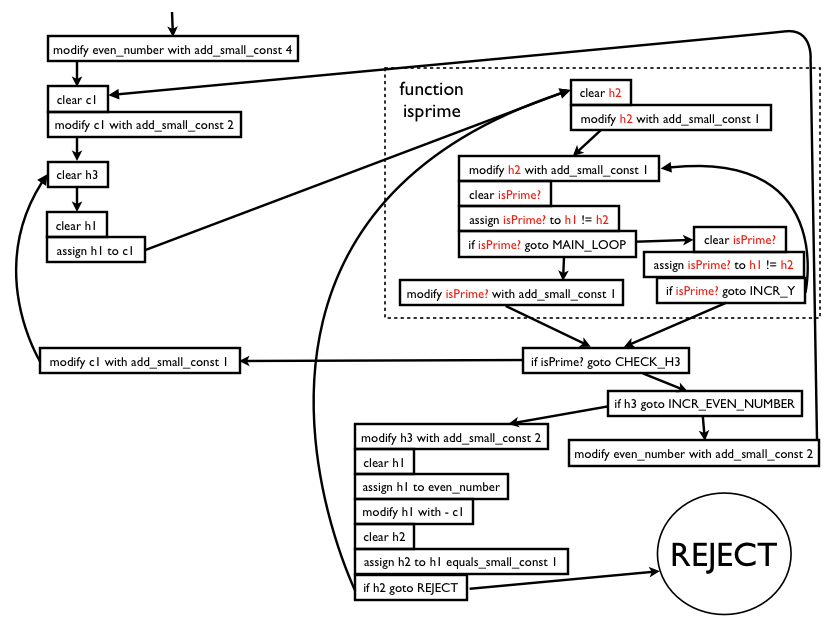
\includegraphics[scale=0.4]{figs/goldbach1.png} 
\caption{A pictorial representation of the compiled output of \texttt{goldbach.tmd}. This state machine will reject if and only if Statement~\ref{goldbachstatement} is false. Each boxed line of code represents a group of states in the multi-tape Turing machine. Arrows from one box to another indicate the state machine's logical flow. When no arrows leave a box, logical flow is presumed to continue to the box immediately beneath it. Note that only \texttt{if} statements cause a branch in the program's logical flow. Note also that the \texttt{isprime} function is inlined directly into the \texttt{goldbach.tmd}. Variable names are shown in red in the \texttt{isprime} function, to indicate that those are the names of the external variables of \texttt{goldbach.tmd}, and not the variables internal to the \texttt{isprime} function. For a more detailed view of the \texttt{isprime} function in which individual states are visible, see Figure~\ref{fig:goldbach2}. \label{fig:goldbach1}}
\end{center} 
\end{figure}

\begin{figure} 
\begin{center} 
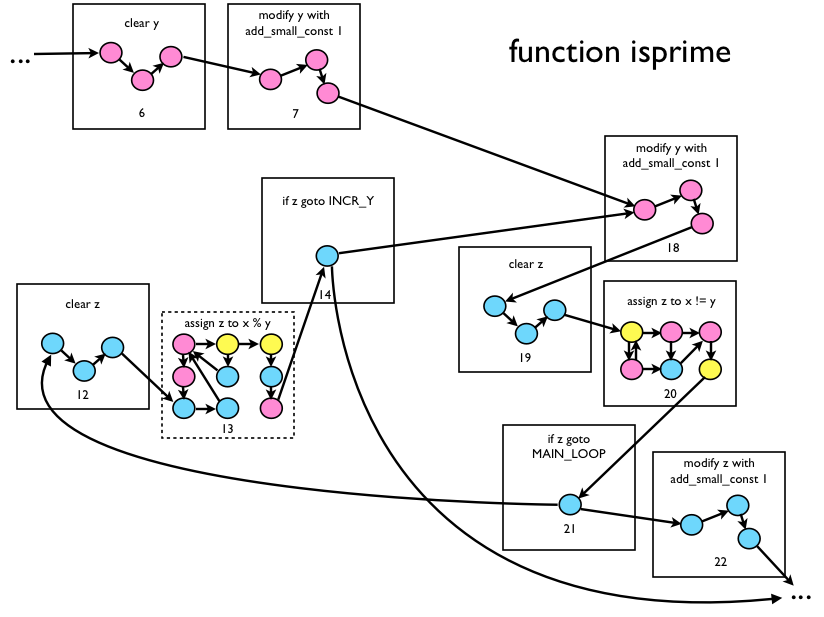
\includegraphics[scale=0.4]{figs/goldbach2.png} 
\caption{A view of the state machine associated with the \texttt{isprime} function, which has as its goal to set the value of $z$ to 1 if $x$ is prime, and set the value of $z$ to 0 otherwise. Each box represents a group of states associated with a line of code in the source of \texttt{isprime.tfn}. The smaller circles represent individual states. Transitions between states are accurate and complete, with two exceptions: transitions from states to themselves and transitions from states to the \texttt{ERROR} state are omitted for clarity. Yellow circles represent states associated with the $x$ tape, pink circles represent states associated with the $y$ tape, and blue circles represent states associated with the $z$ tape. For a more detailed view of the state machine associated with the line of code \texttt{assign z to x \% y}, in which the state transitions are fully described, see Figure~\ref{fig:goldbach3}. \label{fig:goldbach2}}
\end{center} 
\end{figure}

\begin{figure} 
\begin{center} 
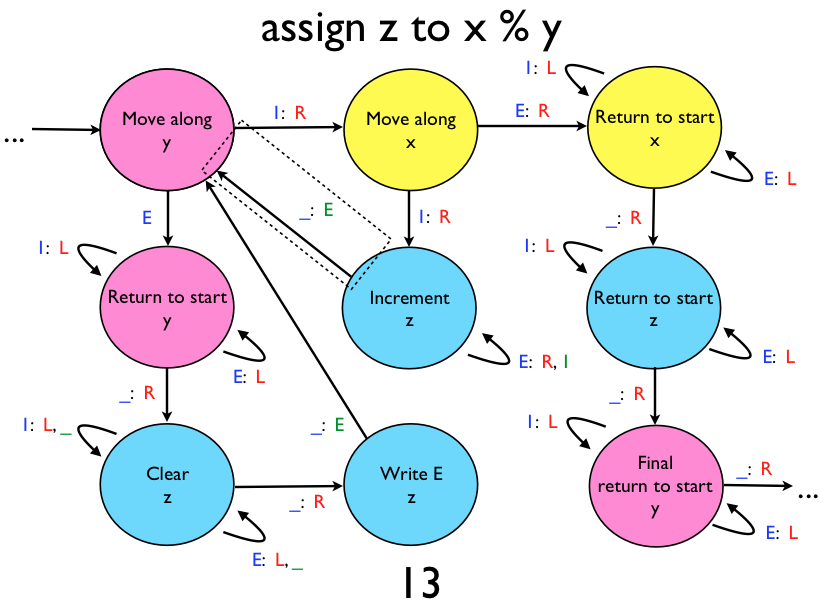
\includegraphics[scale=0.4]{figs/goldbach3.png} 
\caption{A detailed view of the state machine associated with the line of code \texttt{assign z to x \% y} function, which has as its goal to set the value of $z$ to the value $x \mod y$. Each circle represents a state in the multi-tape Turing machine. Transitions between states are accurate and complete, with the exception of transitions from states to the \texttt{ERROR} state, which are omitted for clarity (if there doesn't exist a transition for a given symbol, it can be presumed that that transition is to the \texttt{ERROR} state). Yellow circles represent states associated with the $x$ tape, pink circles represent states associated with the $y$ tape, and blue circles represent states associated with the $z$ tape. On each transition arrow, the character in blue represents the symbol that must be read for this state transition to take place. The character in red represents the direction which the head moves in response to the transition (if omitted, the head remains in place). The character in green represents the new symbol written on the tape (if omitted, the symbol written is the same as the symbol read). To see how a state transition in the multi-tape Turing machine is transformed into its single-tape equivalent, see Figure~\ref{fig:goldbach4}. \label{fig:goldbach3}}
\end{center} 
\end{figure}

\section{Transforming a Multi-Tape Machine into a Single-Tape Machine \label{sec:mttostgoldbach}}

The multi-tape-to-single-tape transformation algorithm transforms the 89-state, 6-tape, 3-symbol Turing machine given in Section~\ref{sec:turdtotmgoldbach} into a 1382-state, single-tape, 4-symbol Turing machine. The details of the transformation algorithm are described in depth in Section~\ref{sec:mttost}. \\

First, a sequence of initialization states are added to the Turing machine, the first of which is the start state. These initialization states write the alternating sequence of identifiers and empty tape values (initialized to \texttt{\_E\_\_\_}\dots, which corresponds to \texttt{0}. The last of the initialization states points to a state corresponding to the start state of the multi-tape Turing machine. From there, the remainder of the algorithm simply takes every state transition in the multi-tape Turing machine, and transforms it using a process described in more detail in Subsection~\ref{mttoststeps}, and shown pictorially in Figure~\ref{fig:goldbach4}.

\begin{figure} 
\begin{center} 
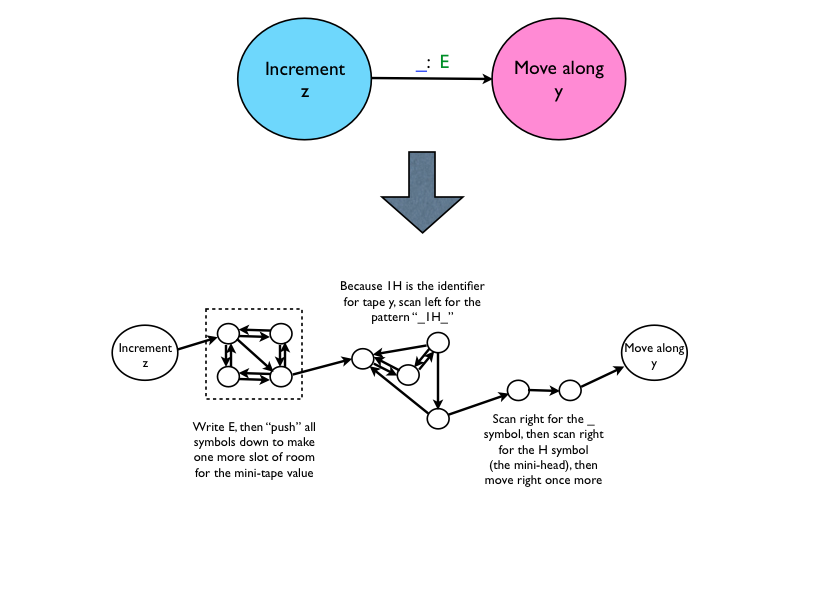
\includegraphics[scale=0.4]{figs/goldbach4.png} 
\caption{A pictorial representation of the multi-tape-to-single-tape transformation algorithm. At the top of the picture is the original state transition: upon reading in a \texttt{\_} symbol, the head on the $z$ tape replaces it with an \texttt{E} symbol and stays in place. At the bottom of the picture is the group of single-tape Turing machine states associated with this multi-tape state transition. Each of the multi-tape states has a single-tape state that directly correspond to it; in between these states are a group of states designed to ``push'' every symbol on the tape down to make more room for the $z$ value, a group of states designed to read in the identifier associated with $y$, and a group of states designed to reach the relevant part of the $y$ tape. In the state machine shown on the bottom, transitions from states to themselves or from states to the \texttt{ERROR} state are omitted. For a more detailed view of the state machine associated with ``pushing down'' every symbol on the tape, see Figure~\ref{fig:goldbach5}. \label{fig:goldbach4}}
\end{center} 
\end{figure}

\begin{figure} 
\begin{center} 
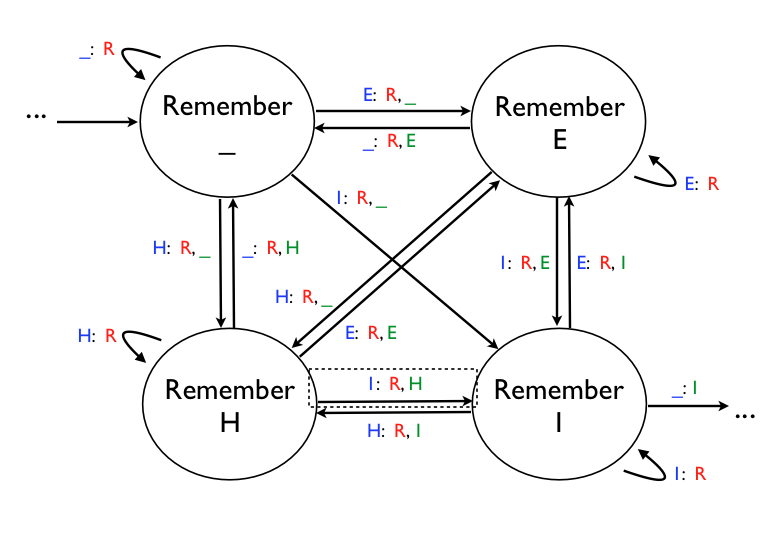
\includegraphics[scale=0.4]{figs/goldbach5.png} 
\caption{A detailed view of the state machine associated with ``pushing down'' every symbol on the tape. Transitions between states are accurate and complete, with the exception of transitions from states to the \texttt{ERROR} state, which are omitted for clarity (if there doesn't exist a transition for a given symbol, it can be presumed that that transition is to the \texttt{ERROR} state). On each transition arrow, the character in blue represents the symbol that must be read for this state transition to take place. The character in red represents the direction which the head moves in response to the transition (if omitted, the head remains in place). The character in green represents the new symbol written on the tape (if omitted, the symbol written is the same as the symbol read). To see how a state transition in the 4-symbol Turing machine is transformed into its 2-symbol equivalent, see Figure~\ref{fig:goldbach6}. \label{fig:goldbach5}}
\end{center} 
\end{figure}

\section{Transforming a 4-Symbol Turing Machine into a 2-Symbol Machine \label{sec:mstotsgoldbach}}

The 4-symbol-to-2-symbol transformation algorithm transforms the 1382-state, single-tape, 4-symbol Turing machine in Section~\ref{sec:mttostgoldbach} into a 7902-state, single-tape, 2-symbol Turing machine. This transformation takes place simply by applying the process described in detail in Section~\ref{sec:mstotssteps} to each of the state transitions in the 4-symbol Turing machine to yield a 2-symbol Turing machine. A pictorial representation of this process is shown in Figure~\ref{fig:goldbach6}.

\begin{figure} 
\begin{center} 
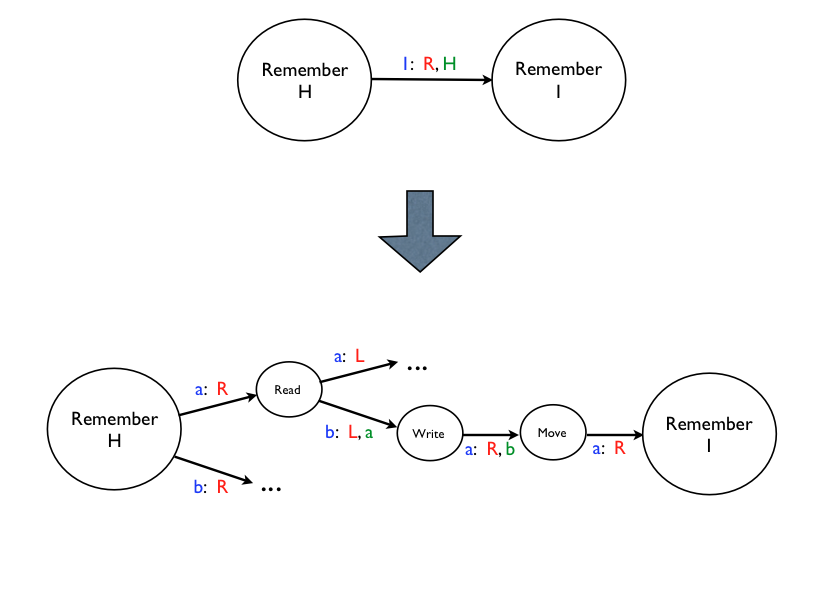
\includegraphics[scale=0.4]{figs/goldbach6.png} 
\caption{A pictorial representation of the 4-symbol-to-2-symbol transformation algorithm. At the top of the picture is the original state transition: upon reading in a \texttt{1} symbol, the head on the $z$ tape replaces it with an \texttt{H} symbol and moves right. At the bottom of the picture is the lower-level state machine. Because a \texttt{1} symbol corresponds to the sequence \texttt{ab} and an \texttt{H} corresponds ot the sequence \texttt{ba}, the lower-level Turing machine is instructed to write the sequence \texttt{ba} on the tape and move right two spaces if the sequence \texttt{ab} is read in. On each transition arrow, the character in blue represents the symbol that must be read for this state transition to take place. The character in red represents the direction which the head moves in response to the transition (if omitted, the head remains in place). The character in green represents the new symbol written on the tape (if omitted, the symbol written is the same as the symbol read). \label{fig:goldbach6}}
\end{center} 
\end{figure}

\begin{thebibliography}{100}
\bibitem{friedman} Friedman, H. ``Order Invariant Graphs and Finite Incompleteness.'' https://u.osu.edu/friedman.8/files/2014/01/FIiniteSeqInc062214a-v9w7q4.pdf
\bibitem{busybeaver} Rado, T. ``On Non-Computable Functions.'' 
Bell System Technical Journal, 41: 3. May 1962 pp 877-884.
\bibitem{bbvalues} http://www.drb.insel.de/~heiner/BB/
\bibitem{codegolf} http://codegolf.stackexchange.com/
\bibitem{grandconjecture} http://cs.nyu.edu/pipermail/fom/1999-April/003014.html
\bibitem{bbimpossible} Marxen, H., Buntrock, J.``Attacking the Busy Beaver 5.'' 
\bibitem{grothendieck} McLarty, C. ``What Does It Take To Prove Fermat's Last Theorem? Grothendieck and the Logic of Number Theory.'' The Bulletin of Symbolic Logic, Volume 00, Number 0.
\bibitem{friedmanlist} Friedman, H. ``Order Theoretic Equations, Maximality, and Incompleteness.'' June 7, 2014. http://u.osu.edu/friedman.8/foundational-adventures/downloadable-manuscripts \#78.
\bibitem{github} https://github.com/adamyedidia/thesis.git
\bibitem{personalcomm} Personal communication between A. Yedidia and H. Friedman.
\end{thebibliography}

\end{document}
% TODO talk about init states
% TODO make underscores bigger
